\documentclass[11pt,a4paper]{article}
\usepackage[margin=1in]{geometry}

% Enter dates of publication

\usepackage{lineno}
\usepackage{graphicx}
\usepackage{authblk}
\renewcommand*{\Authfont}{\bfseries}
\usepackage{hyperref}
\usepackage{comment}
\usepackage[yyyymmdd]{datetime}
\usepackage{makecell}
\usepackage{booktabs}
\usepackage{array}
\renewcommand{\dateseparator}{-}
\newcommand{\gx}[1]{\textcolor{cyan}{#1}}
\newcommand{\methodname}{{\tt{STAnalyzer}}}
\usepackage{float}
% \pagewiselinenumbers
% \raggedbottom


%\articlesubtype{This is the article type (optional)}

\begin{document}



% \title{STAnalyzer: [Explainable and Traceable Spatial Transcriptomics Analysis by an Agentic Architecture]}

\title{STAnalyzer: Transparent Spatial Transcriptomics Analysis via an Agentic Architecture}

\author[1,2,$\dagger$]{Hanwen Luo}
\author[3,$\dagger$]{Liliang Liu}
\author[1,2]{Zhongyu Xing}
\author[1]{Xinlu Li}
\author[1]{Xuerui Zhang}
\author[1,2]{Wei Du}
\author[4,*]{Bin Liu}
\author[2,*]{Jun Wang}
\author[1,2,*]{Guoxian Yu}

\affil[1]{School of Software, Shandong University, Jinan 250101, Shandong, China}
\affil[2]{SDU-NTU Centre for Artificial Intelligence Research, Shandong University, Jinan 250101, Shandong, China}
\affil[3]{Interdisciplinary Center, Shandong University, Jinan 250100, Shandong, China}
\affil[4]{Department of Interventional Medicine and Minimally Invasive Oncology, Shandong University, Jinan 250033, Shandong, China}

\date{
\vspace{0.5cm}
\begin{flushleft}
\small
\textbf{*} To whom correspondence should be addressed. Email: guoxian85@gmail.com. Correspondence may also be addressed to Jun Wang and Bin Liu. Email: kingjun@sdu.edu.cn and gordon0221@163.com.\\
\textbf{$\dagger$} These authors contributed equally to this work.
\end{flushleft}
}

% Affiliation must include:
% Department name, institution name, full road and district address,
% state, Zip or postal code, country


\maketitle

%  感觉没必要强调多智能体是哪几个智能体，直接强调能够做什么
% \begin{abstract}
% Spatial transcriptomics (ST) technologies enable high-resolution profiling of gene expression with spatial context, but their full potential is hindered by fragmented analytical toolchains, complex parameter tuning, and inadequate integration of biological knowledge. Here, we present STAnalyzer (Spatial Transcriptomics Analyzer by Multi-agent Analysis System), an intelligent multi-agent framework designed to streamline end-to-end ST data analysis through autonomous collaboration. STAnalyzer integrates four specialized agents—Orchestrator, Service Planner, Data Interpretation, and Knowledge Integration—operating on a centralized service registry with over 20 standardized bioinformatics tools covering the entire ST analysis lifecycle. The Orchestrator Agent aligns user natural language queries with analytical goals, while the Service Planner Agent translates these goals into executable workflows via dynamic service discovery and automatic parameter configuration.
% To address context overload and fragmented results, the Data Interpretation Agent adopts an ordered reading plan strategy for multi-modal data (text, structured data, images) interpretation. 
% The Knowledge Integration Agent enriches results with external biological knowledge (e.g., PubMed literature, KEGG pathways) and provides traceable evidence. STAnalyzer eliminates manual tool coordination and parameter adjustment, supports reproducible analysis through persistent execution records, and lowers the technical barrier for researchers with varying computational expertise.
% % todo:再加上一些results相关的描述
% This framework enables efficient translation of ST data into biologically meaningful insights, accelerating hypothesis generation and validation in spatial biology research.
% \end{abstract}


% capabilities还是感觉说的有点不足
\begin{abstract}
Spatial transcriptomics enables high-resolution profiling of gene expression within spatial contexts, yet its potential is often hindered by fragmented toolchains, intricate parameters, and cognitive bottlenecks of interpreting high-dimensional data.
While recent Large Language Model agents have attempted to automate this process, they remain constrained by rigid execution logic, lack multimodal feedback for self-correction, and operate in epistemic isolation from established biological knowledge.
Here, we present STAnalyzer, an intelligent multi-agent framework designed to automate the end-to-end analytical lifecycle—from raw data processing to biological hypothesis generation.
Transcending traditional pipelines, STAnalyzer employs a collaborative intelligence architecture to achieve three core capabilities:
(1) \textbf{Intent-Driven Orchestration}, which dynamically translates natural language queries into rigorous bioinformatics workflows; 
(2) \textbf{Multi-Modal Self-Refinement}, which autonomously ensures analytical robustness through closed-loop synthesis of evidence from visual patterns and statistical metrics; and 
(3) \textbf{Evidence-based Cross-Validation}, which bridges the gap between data-driven correlations and biological causation by anchoring findings in ground-truth literature and structured databases.
% todo:再加上一些results相关的描述
% We validated STAnalyzer on ...
By eliminating manual analytical bottlenecks and ensuring rigorous evidentiary traceability and transparency, STAnalyzer makes high-resolution spatial omics more accessible to a broader research community. It provides a robust and scalable framework for cross-platform automated analysis and accelerated biological discovery, translating massive spatial datasets into verifiable biological insights.
\end{abstract}

\begin{figure*}
    \centering
    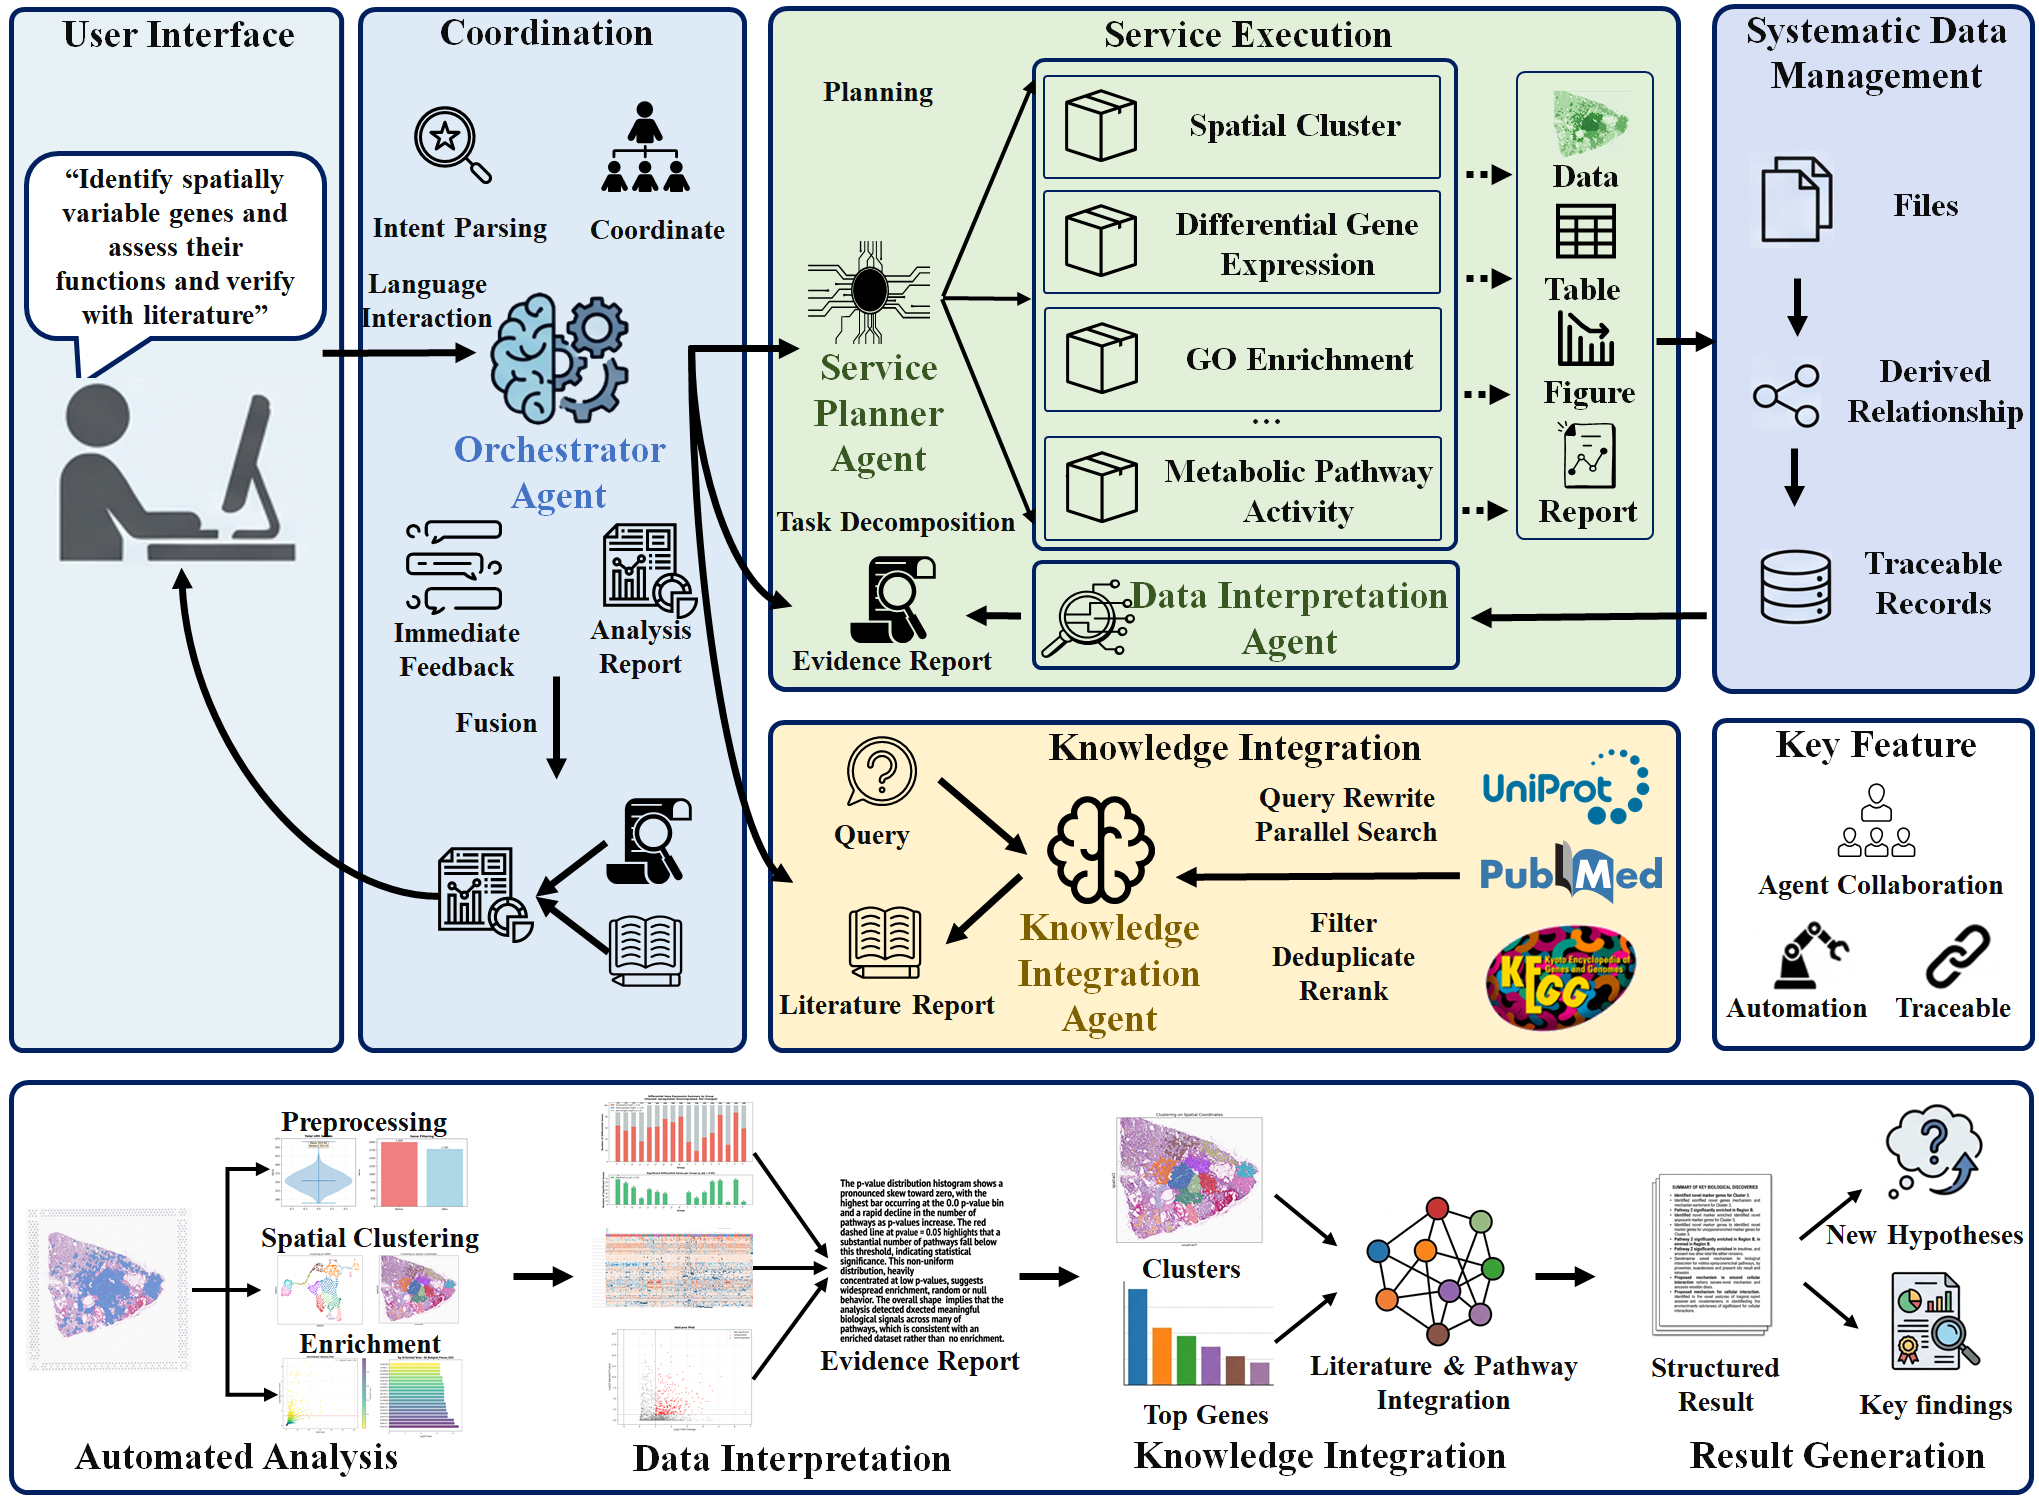
\includegraphics[width=1\linewidth]{figure/Architecture_of_System.png}
    \caption{System architecture and end-to-end workflow of STAnalyzer. The framework comprises: (1) a natural language User Interface; (2) the Orchestrator Agent for intent parsing and multi-agent coordination; (3) the Service Execution layer including the Service Planner Agent, specialized analytical services, and the Data Interpretation Agent; (4) the Knowledge Integration Agent linking external resources (PubMed, KEGG); (5) the Data Management module for file provenance and traceability; and (6) an end-to-end workflow from automated analysis through knowledge integration to result generation. 
    % \gx{[The four main agents should be highlighted with non-black color]
    % }
    }
\label{fig:stamas_architecture}
\end{figure*}

\section{Introduction}
Spatial transcriptomics (ST) has emerged as a transformative technology in modern biology and medicine, enabling the simultaneous capture of gene expression profiles and their spatial contextualization within intact tissues \cite{rao2021exploring,marx2021method}. This unique capability has unlocked unprecedented insights into tissue architecture, cellular crosstalk, developmental dynamics, and disease microenvironment heterogeneity, revolutionizing fields ranging from basic developmental biology to precision oncology and neuroscience \cite{maynard2021transcriptome,xia2025deciphering}. With the rapid advancement of ST platforms (e.g., Visium, Slide-seq \cite{rodriques2019slide}, and MERFISH \cite{chen2015spatially}), the volume of spatial transcriptomic data has grown exponentially, driving an urgent demand for efficient, standardized, and user-friendly analytical tools \cite{moses2022museum}.

% 现在有很多对空转数据提供的数据库以及平台，但是对于空转数据分析对于从业者有着很高的要求（现有工具繁多、部署环境的复杂、以及对于结果的读取以及理解）
While platforms like SpatialRef \cite{cui2025spatialref} and SODB \cite{yuan2023sodb} provide essential ST resources, their practical utility is hindered by dual technical and cognitive bottlenecks. Computationally, fragmented pipelines and complex deployments present significant challenges for biologists lacking advanced computational expertise \cite{fang2023computational,dries2021giotto,palla2022squidpy}. Biologically, deciphering high-dimensional outputs into actionable insights demands substantial domain knowledge, imposing a considerable cognitive load. Furthermore, current isolated tools intrinsically lack cross-step, cross-result, and context-aware interpretive capabilities. Consequently, this limited systemic integration, coupled with steep knowledge prerequisites, constrains the broader application of ST technologies. 

% However, the analysis of spatial transcriptomic data remains a formidable challenge. First, the integration of spatial information with high-dimensional genomic data requires specialized bioinformatics expertise, creating a significant technical barrier for researchers without advanced computational training. Second, the lack of standardized analytical pipelines has led to fragmented workflows, where data processing, quality control, downstream analysis (e.g., clustering, spatial domain identification, pathway enrichment), and biological interpretation are often performed using disjointed tools, resulting in reduced reproducibility and transparency. Third, existing solutions fail to address the full lifecycle of ST data analysis: while databases and toolkits such as SpatialRef (Cui et al., 2025, Nucleic Acids Res.), STOmicsDB (Xu et al., 2024, Nucleic Acids Res.), and SODB (Yuan et al., 2023, Nat. Methods) provide valuable resources for data storage and specific analytical modules, they lack end-to-end integration from raw data processing to biological hypothesis generation. Recent advances in natural language-driven tools, including PromptBio (Zhang et al., 2025, bioRxiv) and Biomni (Huang et al., 2025, bioRxiv), have simplified user interactions but still fall short in supporting critical full-cycle services—such as intermediate result validation, context-aware biological interpretation, literature-based verification, and extraction of novel mechanistic insights.

\enlargethispage{-65.1pt}
% 明天重新调整这一段
In recent years, the breakthrough progress of Large Language Models (LLMs) in zero-shot learning and generalization has significantly advanced bioinformatics and automated experimental data analysis, inspiring representative works such as Cell Agent \cite{xiao2024cellagent}, Bio Agents \cite{mehandru2025bioagents}, and Bioinformatics Agents \cite{xin2024bioinformatics} to build intelligent agents for complex task automation. However, applying these general-purpose bio-agents to spatial transcriptomics data reveals critical deficiencies in handling real-world scientific complexity. First, existing methods often suffer from fragile execution without dependency awareness, as they treat bioinformatics tools as isolated entities while neglecting the implicit logical dependencies between analytical steps and the volatility of fragmented ecosystems \cite{dries2021giotto,liu2025benchmarking}; Second, current systems are characterized by open-loop execution with multimodal blindness, operating as "fire-and-forget" pipelines that lack the semantic capability to interpret multimodal outputs \cite{wang2025large}. Without a structured strategy to navigate complex results, these agents frequently succumb to context overflow and fail to perform essential self-reflection or dynamic replanning based on intermediate biological signals. Third, these agents suffer from epistemic isolation from external knowledge because they rely on static internal parameters, which prevents them from synergizing structured databases with unstructured literature. Lacking mechanisms for query alignment or coarse-to-fine reading, they cannot retrieve high-fidelity evidence, rendering them unable to provide the traceable, citation-backed insights required to distinguish genuine biological discoveries from technical artifacts \cite{neha2025retrieval}.

% \newpage
% \begin{itemize}
%     \item \textbf{Fragile Execution without Dependency Awareness:} Existing methods treat bioinformatics tools as isolated tools, neglecting the implicit logical dependencies between analytical steps and the volatility of fragmented ecosystems \cite{dries2021giotto,liu2025benchmarking}. This oversight regarding library versioning and environmental configurations leads to logically disjointed plans and frequent execution failures intrinsic to heterogeneous environments.
%     \item \textbf{Open-Loop Execution with Multimodal Blindness:} Current systems operate as `fire-and-forget' pipelines, lacking the semantic capability to interpret multimodal outputs \cite{wang2025large}. Without a structured strategy to navigate complex results, these agents suffer from context overflow and fail to perform self-reflection or dynamic replanning based on intermediate biological signals.
%     \item \textbf{Epistemic Isolation from External Knowledge:} Relying on static internal parameters, agents fail to synergize structured databases with unstructured literature. Lacking mechanisms for query alignment or coarse-to-fine reading, they cannot retrieve high-fidelity evidence, rendering them unable to provide the traceable, citation-backed insights required to distinguish biological discoveries from technical artifacts \cite{neha2025retrieval}.
% \end{itemize}

% 为此，我们构建了STAnalyzer，一个多agent协作的框架用户仅需要将数据以及自然语言的查询交给STAnalyzer，其即可自动产生相关的生信分析计划，并且在每一步调用相关的生信分析服务，得到相关结果（包括图像、统计信息以及图表等），并对结果进行分析，总结其中关键的生物学发现，评估当选执行步骤是否合理，符合预期，并且对于找到的关键间接，检索并读取相关的科研文献，向用户给出有意义的结果。
% 1/11 计划后续再加入我们提供的前端页面的叙述
% To bridge these critical gaps, we present STAnalyzer, an intelligent multi-agent collaborative framework designed to automate spatial transcriptomics analysis. STAnalyzer allows researchers to interface with complex ST data through natural language. By simply providing raw data and a research query (e.g., ``Identify genes driving the tumor microenvironment changes and verify with literature''), users can trigger an autonomous analytical lifecycle. To ensure rigor and accessibility, STAnalyzer integrates three core capabilities:
% \begin{itemize}
%     \item \textbf{Autonomous Planning and Orchestration:} The system decomposes high-level intents into executable bioinformatics workflows. It autonomously schedules tasks—from data normalization to spatial clustering—and invokes relevant tools to generate multimodal outputs, including statistical summaries and high-dimensional visualizations.
%     \item \textbf{Self-Refining Quality Assurance:} Transcending standard automation workflows, STAnalyzer employs a closed-loop feedback mechanism. It critically evaluates intermediate results against analytical standards (e.g., verifying clustering separation) and autonomously rectifies parameters to ensure robust outcomes.
%     \item \textbf{Evidence-based Cross-Validation:} To validate biological plausibility, STAnalyzer integrates a dual-pipeline knowledge engine. It cross-references internal computational findings against external ground truth retrieved from structured databases and high-impact literature. This process generates traceable, citation-backed insights, effectively bridging the gap between data-driven inference and biologically established causation.
% \end{itemize}
% By automating and enhancing the traceability of the lifecycle of ST data analysis, STAnalyzer effectively lowers the technical barrier, ensures the traceability of the analysis process, and substantially reduces the cognitive load required for researchers to translate high-dimensional computational outcomes into biological discoveries.

To bridge these critical gaps, we present STAnalyzer, an intelligent multi-agent collaborative framework designed to automate the spatial transcriptomics analysis lifecycle through natural language interaction. By simply providing raw data and a research query (e.g., ``Identify genes driving the tumor microenvironment changes and verify with literature"), users trigger an autonomous process that integrates three core capabilities. First, the system excels in autonomous planning and orchestration, decomposing high-level intents into executable bioinformatics workflows that range from data normalization to the generation of multimodal visualizations. Second, STAnalyzer employs self-refining quality assurance through a closed-loop feedback mechanism, critically evaluating intermediate results against analytical standards and autonomously rectifying parameters to ensure robust outcomes. Third, the framework performs evidence-based cross-validation via a dual-pipeline knowledge engine that cross-references computational findings with external ground truth from structured databases and high-impact literature. This process generates traceable, citation-backed insights that bridge the gap between data-driven inference and established biological causation. By automating and enhancing the entire analytical pipeline, STAnalyzer effectively lowers technical barriers, ensures process traceability, and substantially reduces the cognitive load required to translate high-dimensional outcomes into meaningful biological discoveries. Through applications on both spot-level and subcellular-resolution spatial transcriptomic datasets encompassing human brain and lung cancer, STAnalyzer demonstrates its effectiveness in two complementary dimensions: rapidly and autonomously recapitulating established biological paradigms, and serving as a scalable engine for cross-platform automated analysis and accelerated biological discovery.

% 介绍STAnalyzer实现了什么功能，怎么实现的
\section{Materials and methods}
% \subsection{Multi-agent Collaborative Framework of STAnalyzer}
% STAnalyzer is an intelligent multi-agent collaborative system tailored for comprehensive and end-to-end ST data analysis. STAnalyzer decomposes complex biological analysis workflows into transparent, verifiable atomic pipelines, which are orchestrated through four functionally specialized and human-interpretable agent roles: the \textbf{Orchestrator Agent} (OA), \textbf{Service Planner Agent} (SPA), \textbf{Data Interpretation Agent} (DIA), and \textbf{Knowledge Integration Agent} (KIA). The core design enables users to input high-level research intentions via natural language, with the system autonomously coordinating specialized agents, managing intermediate files and execution states, and ultimately delivering biologically meaningful, traceable analytical results.
% Beyond the autonomous multi-agent architecture, STAnalyzer integrates an interactive visualization interface designed to facilitate \textbf{Human-in-the-Loop} (HITL) analytics. This interface empowers researchers with fine-grained control over the analytical lifecycle, allowing them to transition from passive observers to active collaborators. Specifically, it supports real-time workflow intervention, manual task execution and re-execution, and the modular invocation of individual agents for targeted investigations. This hybrid approach ensures that computational autonomy is seamlessly augmented by human domain expertise, mitigating the `black-box' nature of traditional AI systems.

\subsection{STAnalyzer Architecture: A Human-in-the-Loop Multi-Agent Framework}
STAnalyzer is an intelligent collaborative system tailored for comprehensive spatial transcriptomics (ST) data analysis. In contrast to traditional ``black-box'' automated pipelines, STAnalyzer implements a \textbf{Human-in-the-Loop (HITL)} paradigm, seamlessly integrating multi-agent autonomy with human domain expertise. The core engine is orchestrated through four functionally specialized agents: the \textbf{Orchestrator Agent} (OA), \textbf{Service Planner Agent} (SPA), \textbf{Data Interpretation Agent} (DIA), and \textbf{Knowledge Integration Agent} (KIA). These agents autonomously decompose complex biological workflows, manage execution states, and query external knowledge. However, rather than operating in isolation, the framework embeds the user at the center of the decision-making process, ensuring that computational autonomy is continuously guided, verified, and refined by human intuition.
% 感觉HITL还是放在第一段会比较好，突出我们系统整体的架构，页面范式，表示我们不仅是一个简单的多智能体

% 之后结合图修改一下
\subsection{Interactive Human-in-the-Loop (HITL) Interface}

This synergistic architecture is operationalized via a web-based dashboard that establishes a continuous human--AI collaborative loop. Within this interface, the analytical workflow is represented as a dynamic provenance graph. Researchers can select specific intermediate data nodes from this graph and integrate them into the conversational context. While natural language prompts can trigger the agents to autonomously parse requirements and execute bioinformatics workflows, the system strictly maintains process transparency. When granular intervention is required, researchers can override agent autonomy to manually configure execution parameters, define analytical boundaries, and initiate specific services. As intermediate outputs are generated, they can be dynamically reassigned as new context, enabling an iterative, query-driven exploration of the data. 

To bridge computational results with biological interpretation, the interface integrates essential spatial visualization capabilities. This allows users to inspect key spatial characteristics, such as cell distribution patterns, gene expression heterogeneity, and spatial co-localization, directly within the analytical context. By cross-referencing these visual cues with agent-generated structured reports and retrieved literature, users can critically evaluate the validity of the computational findings. Ultimately, this mechanism establishes a rigorous analytical loop: system output triggers human verification, which in turn guides subsequent computational interventions and optimizations. If the results deviate from biological expectations, the workflow can be seamlessly rolled back to previous decision nodes for re-evaluation. Ultimately, this HITL design culminates in the delivery of a comprehensive and fully traceable analytical report.

\subsection{Orchestrator Agent (OA): User-Centric Coordinator}
As the sole user-facing entry point and central coordinator of STAnalyzer, the OA functions as a user proxy responsible for translating unstructured natural language requests into structured, executable actions while maintaining global analytical consistency. Upon parsing a user’s research intent, the OA iteratively manages the system by mapping high-level goals to concrete bioinformatics tasks—such as data normalization or spatial domain identification—via explicit service execution directives. Beyond mere task delegation, it actively evaluates execution outcomes and intermediate data files through result inspection and feedback parsing, determining whether current analytical objectives are met or require parameter rectification. This technical workflow is further enriched by knowledge retrieval and integration, which triggers KIA queries to bridge the gap between data statistics and biological significance using external databases and literature. Throughout this lifecycle, the OA anchors the process within a dynamic Global Context Memory—logging project background, data states, and historical interactions—to ensure that every analytical step remains tightly aligned with the user’s scientific hypothesis until a comprehensive, biologically grounded result is achieved.
% OA serves as the sole user-facing entry point of STAnalyzer, functioning as a user proxy and central orchestrator. Its core responsibility is to translate unstructured user natural language requests into structured, executable agent actions and maintain the global consistency of the analytical process.

% Upon parsing the user’s research intent, OA iteratively coordinates the system through three types of structured task instructions:
% \begin{enumerate}
%     \item \textbf{Service Execution:} Based on the logical decomposition of the research goal, the OA issues explicit instructions to specialized agents (e.g., the SPA). These directives map high-level intents to concrete bioinformatics tasks, such as data normalization, spatial domain identification, or differential expression analysis.
    
%     \item \textbf{Result Inspection and Feedback Parsing:} Rather than passively waiting for completion, the OA actively engages in reading and evaluating execution outcomes. It parses structured feedback from the SPA and inspects intermediate data files (e.g., interpreting cluster separation in a CSV or identifying anomalies in a spatial plot) to check whether the current step satisfies \textbf{analytical objectives} or requires parameter adjustment.

%     \item \textbf{Knowledge Retrieval and Integration:} To bridge the gap between data statistics and biological meaning, the OA triggers knowledge queries and directs KIA to retrieve external biological context, including marker gene annotations, pathway databases, and relevant literature, to explain analytical findings and refine subsequent planning.
% \end{enumerate}

Throughout this process, the OA maintains a dynamic Global Context Memory, which logs project background, uploaded data states, and historical interaction records. By continuously cycling, inspecting results, and querying knowledge, the Orchestrator ensures that the analysis not only progresses technically but also aligns tightly with the user's scientific hypothesis until a comprehensive, biologically meaningful final result is generated.


\subsection{Service Planner Agent (SPA): Addressing Bioinformatics Complexity in Tool Selection and Execution Robustness}

\begin{figure*}
    \centering
    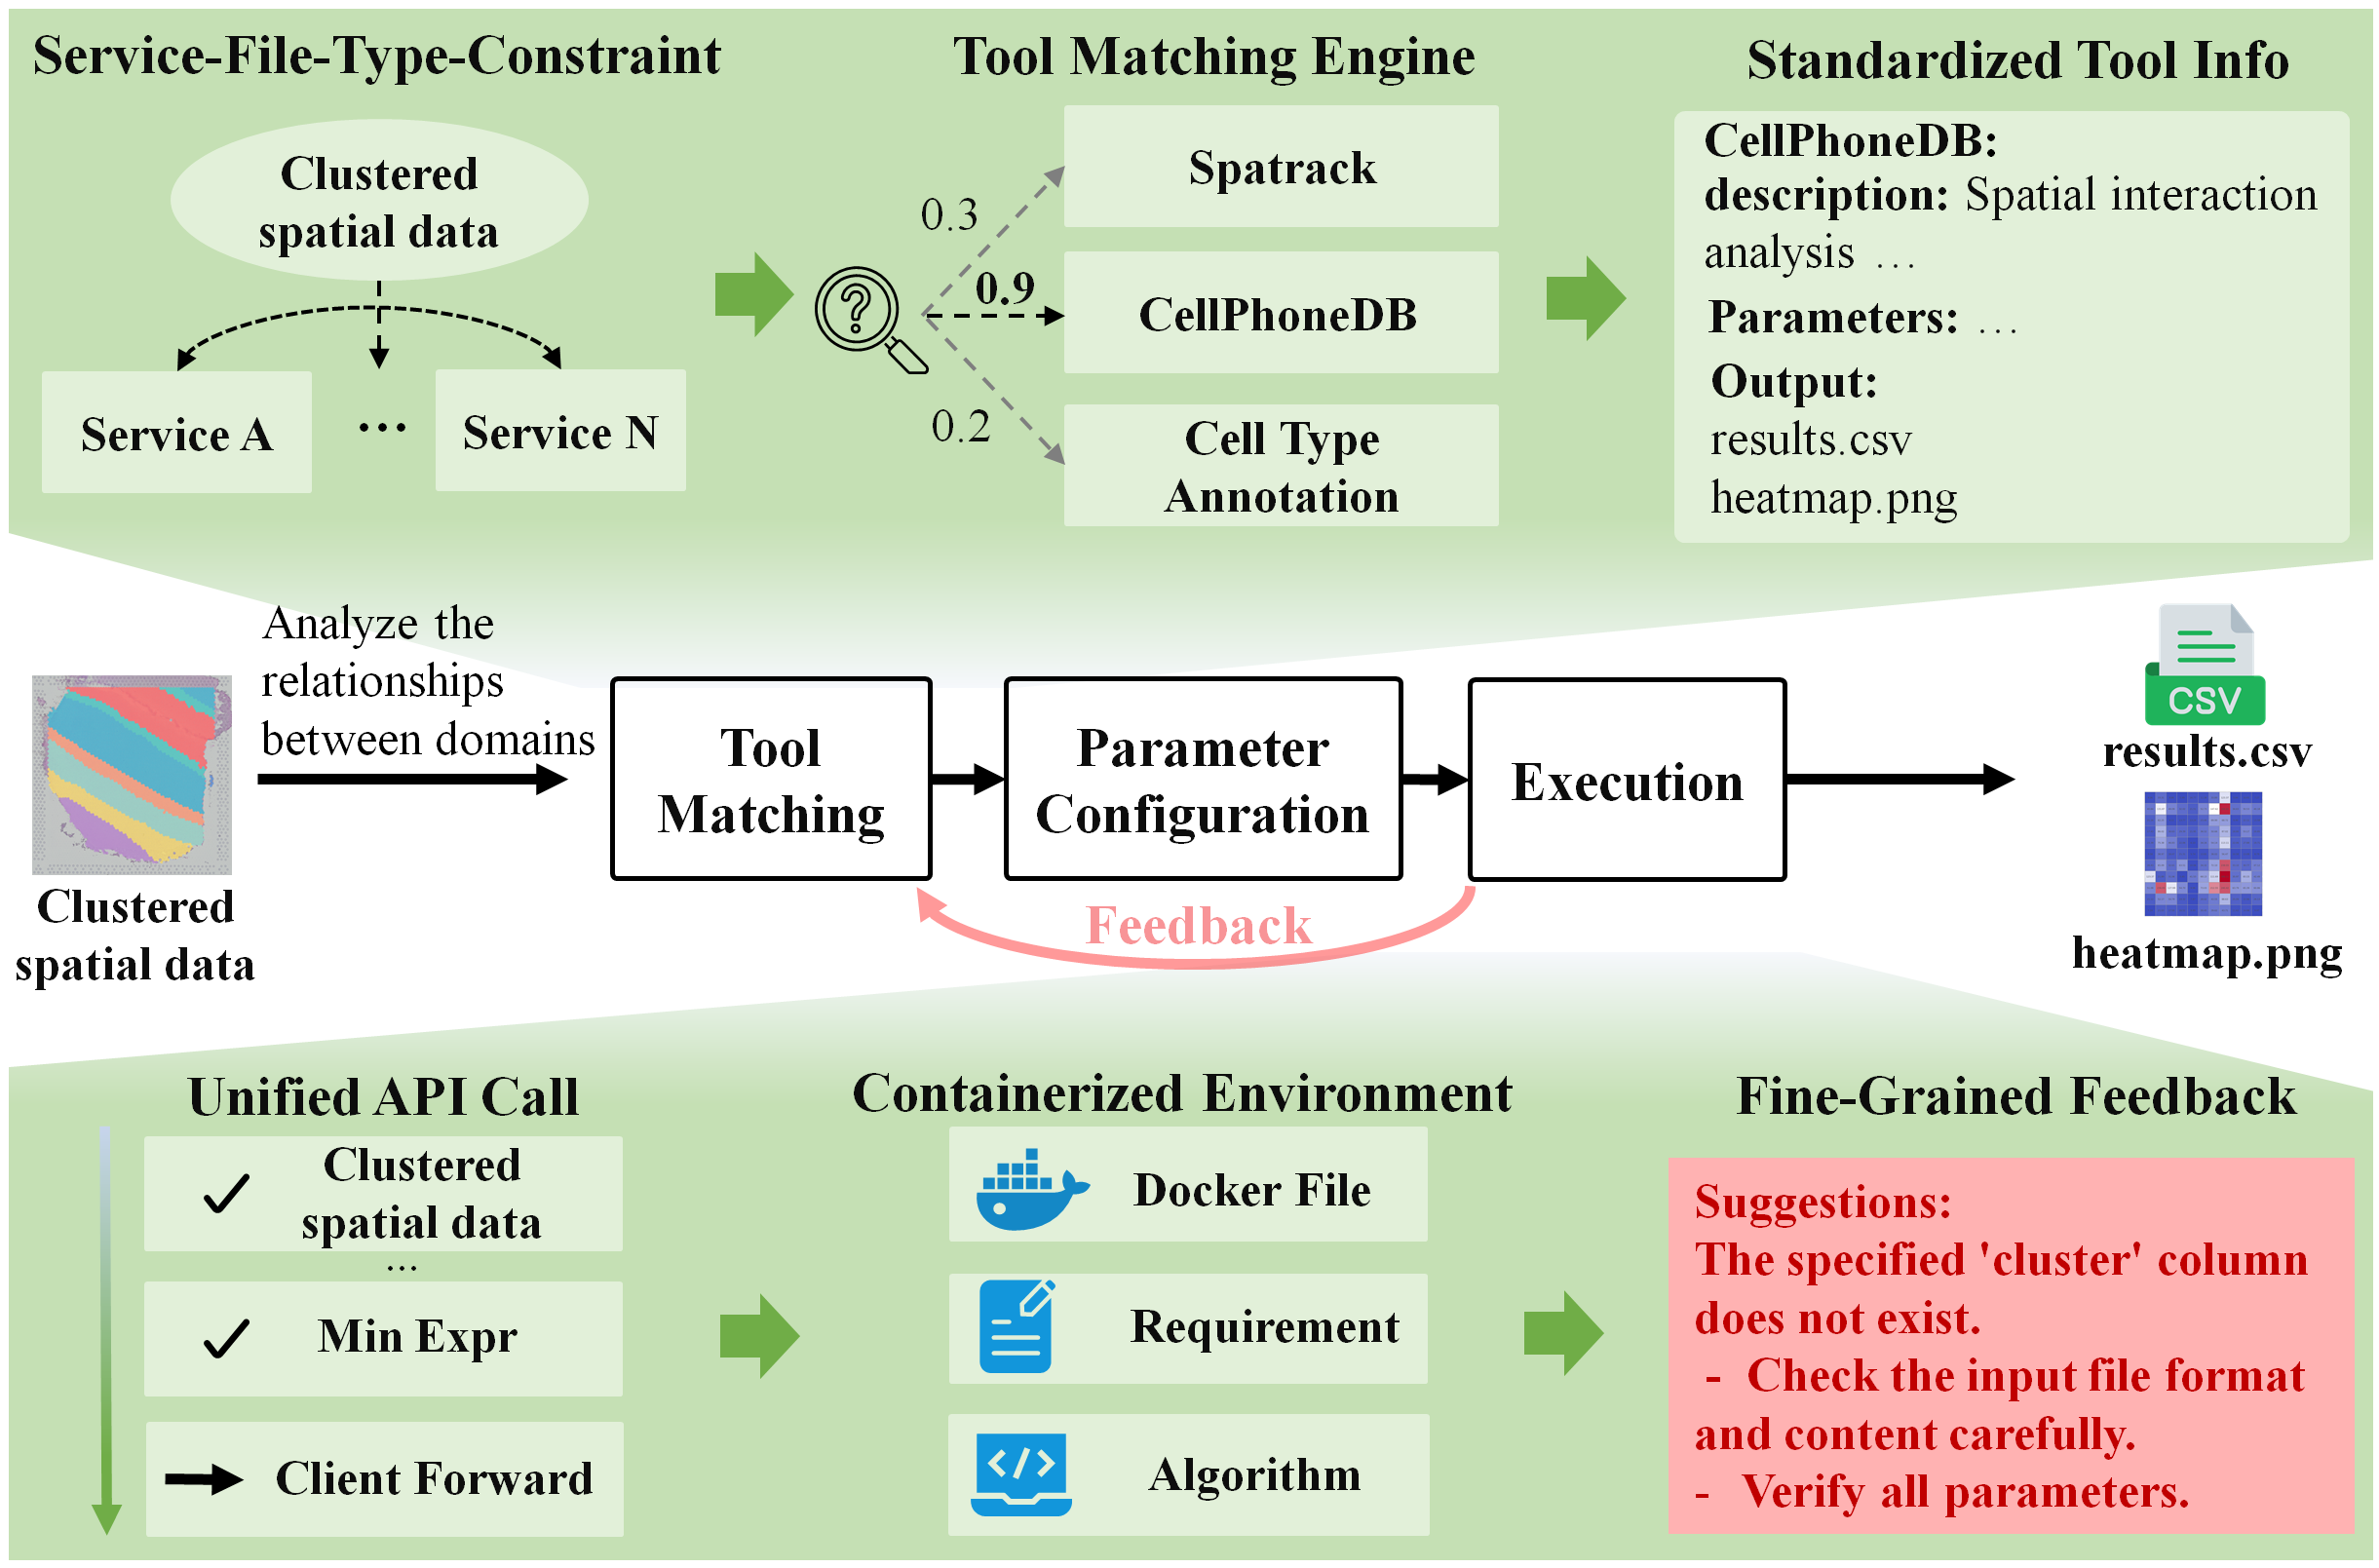
\includegraphics[width=1\linewidth]{figure/Architecture_of_the_Service_Planner_Agent.png}
    \caption{\textbf{Architecture of the Service Planner Agent.} The framework is organized into three logical layers: (Top) The \textbf{Tool Matching Layer} leverages Service-File-Type Constraints and a semantic Tool Matching Engine to select appropriate tools (e.g., CellPhoneDB) based on standardized descriptions. (Middle) The \textbf{Execution Workflow Layer} illustrates the closed-loop process from tool matching and parameter configuration to execution, incorporating a feedback mechanism for error recovery. (Bottom) The \textbf{Infrastructure Layer} supports the workflow via a Unified API Call interface and a Containerized Runtime Environment, providing Fine-Grained Diagnostic Feedback to resolve execution failures.}
    \label{fig:service_planner_agent}
\end{figure*}

SPA is designed to translate abstract research intents into concrete, reliable analytical steps, but its application in bioinformatics is hindered by significant challenges. Specifically, the agent must navigate a vast tool selection space complicated by implicit task dependencies, manage intrinsically unstable execution environments prone to complex programming language and library compatibility issues, and overcome cryptic diagnostic feedback that severely limits its ability to devise effective error recovery strategies. To systematically resolve these interconnected planning, execution, and debugging bottlenecks, we propose a three-layer framework that integrates constraint matching, a robust execution loop, and containerized microservices to ensure seamless and automated analysis.

% SPA is designed to instantiate abstract research intents, converting generalized task assignments into concrete, reliable analytical steps. However, performing this translation in bioinformatics faces three core challenges:

% \begin{enumerate}
% \item \textbf{Vast Tool Selection Space with Implicit Dependencies:} Analytical tasks (e.g., Enrichment Analysis) often depend on prerequisite steps such as Differential Expression Analysis or Functional Domain Identification. This forces the agent to navigate a vast toolset while accounting for implicit task dependencies, significantly increasing the planning complexity and uncertainty.

% \item \textbf{Complex Execution Environment and Compatibility Challenges:} Bioinformatics tools rely on diverse programming environments (e.g., Python, R, Perl) and specific library versions. This diversity renders tool deployment and version control notoriously complex, easily triggering environment incompatibility errors and making the execution layer intrinsically unstable.

% \item \textbf{Insufficient Fine-Grained Diagnostic Feedback:} When an analytical tool fails, the agent typically receives only cryptic stack traces. The lack of precise root-cause diagnostics (e.g., improper parameter settings, input data quality issues) hampers the agent’s ability to devise effective recovery strategies (e.g., automatic parameter adjustment, pipeline replacement), leading to analysis interruption or futile retries.
% \end{enumerate}

To systematically address these challenges, we propose a three-layered framework (Figure \ref{fig:service_planner_agent}), integrating constraint-based matching, a robust execution loop, and containerized microservices.

\textbf{Constraint-based Tool Matching (Top Layer):} To navigate the expansive toolset, we establish a Service-File-Type Constraint mechanism. As shown in the top panel of Figure \ref{fig:service_planner_agent}, this mechanism first constrains the search space based on the input data type (e.g., mapping ``Clustered spatial data'' to candidate tools like spatrack and CellPhoneDB). Subsequently, the Tool Matching Engine evaluates these candidates against the user's specific intent. By comparing the intent with \textbf{Standardized Tool Info}, the engine assigns relevance probabilities—for instance, assigning a high confidence score of 0.9 to CellPhoneDB for interaction analysis tasks, while assigning lower scores (e.g., 0.2 or 0.3) to less relevant tools.

\textbf{Robust Execution Workflow (Middle Layer)}: 
The middle panel of Figure \ref{fig:service_planner_agent} illustrates the agent's robust execution workflow, which operates as a closed loop explicitly driven by both data and research intent. Upon receiving input data, the agent first utilizes a Matching Engine to select the optimal analytical tool and configures its parameters based on standardized metadata. The task is then dispatched through a unified API call, ensuring standardized interaction regardless of the underlying programming language, such as R or Python. Following execution, the system either generates successful analytical results or, in the event of a failure, activates a continuous feedback mechanism that captures fine-grained diagnostic information. This feedback loop empowers the agent to iteratively adjust parameters or re-plan the analysis, significantly enhancing its overall robustness against runtime errors.

% \textbf{Robust Execution Workflow (Middle Layer)}: 
% The middle panel of Figure \ref{fig:service_planner_agent} illustrates the agent's closed-loop operation, which is explicitly driven by both data and research intent via a closed-loop workflow:
% \begin{enumerate}
%     \item \textbf{Tool Matching \& Configuration:} The agent receives data (e.g., Clustered spatial data) and uses the Matching Engine to select the optimal tool, subsequently configuring parameters based on the tool's standardized metadata.
%     \item \textbf{Execution via Unified API:} The task is dispatched through a unified API call, ensuring standardized interaction regardless of the underlying language (R/Python).
%     \item \textbf{Feedback-Driven Loop:} Upon successful execution, results (e.g., CSVs, Heatmaps) are generated. If execution fails, the Feedback loop captures the fine-grained diagnostic information to adjust parameters or re-plan, significantly enhancing robustness against runtime errors.
% \end{enumerate}

\textbf{Containerized Microservices with Fine-Grained Feedback (Bottom Layer)}:
To resolve environment fragility, we refactored bioinformatics tools into a Microservices Architecture. As illustrated in the bottom panel of Figure \ref{fig:service_planner_agent}, tasks are dispatched via unified API call, which encapsulates the data and parameters (e.g., \texttt{Min expr}). Each tool runs within an isolated containerized runtime environment (defined by Dockerfile and Requirements). Crucially, the system replaces cryptic stack traces with fine-grained feedback. For example, when a ``cluster label column not found'' error occurs, the system generates structured suggestions (e.g., ``Check input file format'', ``Verify parameters''), enabling the agent to pinpoint the root cause (e.g., column name mismatch) rather than blindly retrying.

Furthermore, the agent incorporates mechanisms to identify similar failure patterns, ensuring that non-productive execution cycles are terminated after repeated failures, redirecting the process to result reporting, thus guaranteeing system stability and reliability. For customized needs beyond the scope of predefined tools, SPA also supports generating and executing customized analysis scripts in a secure isolated environment, integrating the results into the overall analytical sequence.

\begin{figure*}
    \centering
    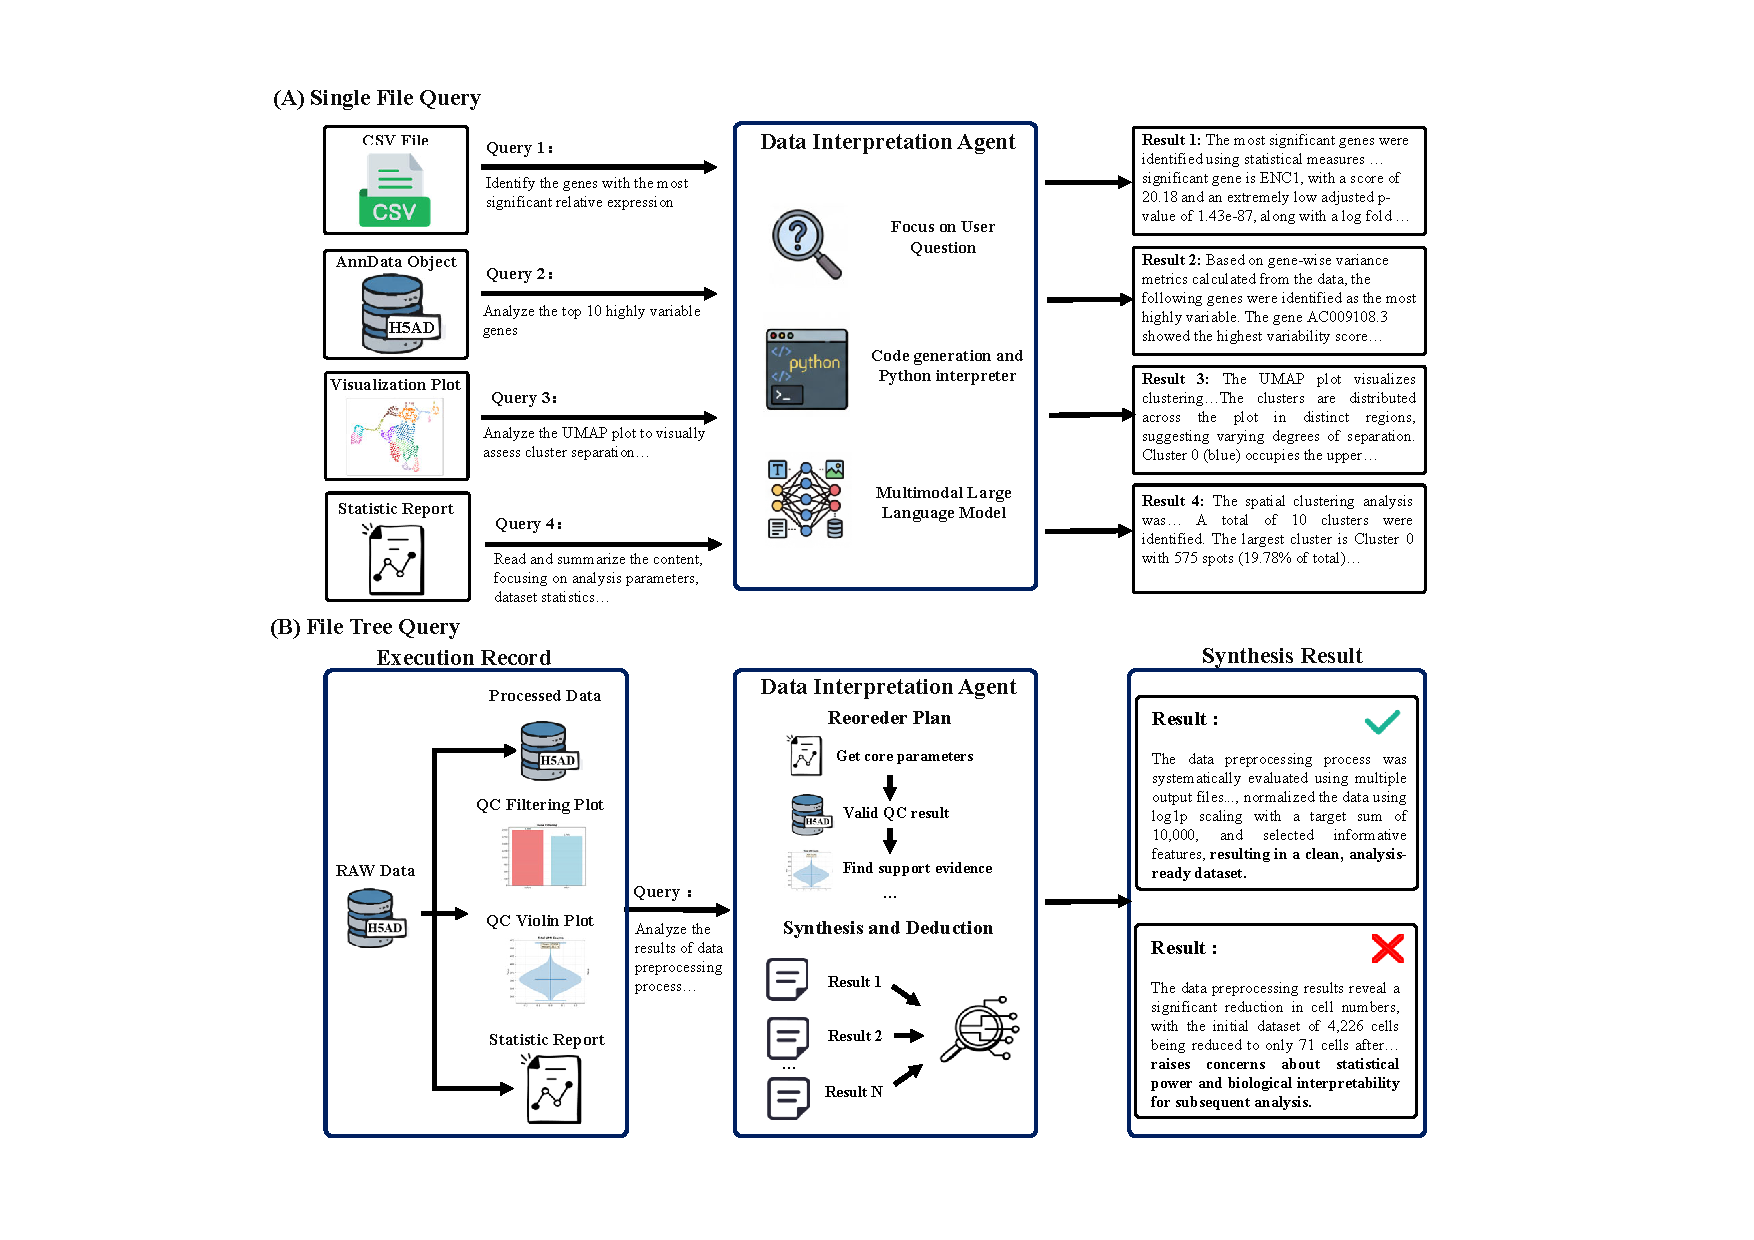
\includegraphics[width=1\linewidth]{Data-Interpretation-Agent.pdf}
    \caption{\textbf{Workflow of the Data Interpretation Agent.} 
    \textbf{(A) Single File Query:} The agent processes individual files (CSV, H5AD, Images, Reports, etc.) based on specific user queries. It utilizes tools like code interpreters and multimodal models to extract gene signatures, statistical metrics, and visual cluster patterns.
    \textbf{(B) File Tree Query:} For complex synthesis tasks, the agent inputs the entire execution record. It employs a ``Reorder Plan" to prioritize data access (e.g., getting parameters before evidence), performs synthesis and deduction, and outputs a final validation result (Pass/Fail) regarding the analysis quality.}
    \label{fig:Data-Interpretation-Agent}
\end{figure*}

% todo:还需要规范化一些,可能再加上description？
% \begin{table*}[htbp]
% \centering
% \small
% \setlength{\tabcolsep}{8pt} % 调整列间距
% \begin{tabular}{@{}p{0.25\textwidth}|p{0.7\textwidth}@{}} % 全宽分配列宽
% \toprule
% \textbf{Service Category} & \textbf{Specific Services} \\
% \midrule
% Preprocessing & spatial-transcriptomics-preprocessing, single-cell-preprocessing \\
% Clustering and domain detection & spatial-domain-detection-squidpy, banksy-service, spaotsc-service \\
% Differential expression & spatial-dge, spatial-variation-analysis \\
% Deconvolution and imputation & spatial-deconvolution-cell2location-service, spatial-imputation-spage-service, spatial-imputation-tangram-service \\
% Trajectory inference & spatial-trajectory \\
% Cell-cell interaction & cellphonedb-service, giotto-cpdb-service, nichenet-service, misty-service \\
% Gene regulatory networks & scdgrn-service, celloracle-perturbation-service, sctenifoldpy-knockout-service \\
% Functional enrichment & gene-enrichment-analysis \\
% Cell type annotation & singler-annotation, spatial-marker-gene-annotation \\
% Spatial analysis & spatialde, spatial-metabolic-activity-service \\
% \bottomrule
% \end{tabular}
% \caption{Summary of specialized bioinformatics services integrated in STAnalyzer, covering the full lifecycle of spatial transcriptomics analysis. All services follow standardized interfaces and are accessible via the system’s service registry.}
% \label{tab:stamas_services}
% \end{table*}

\begin{figure*}
    \centering
    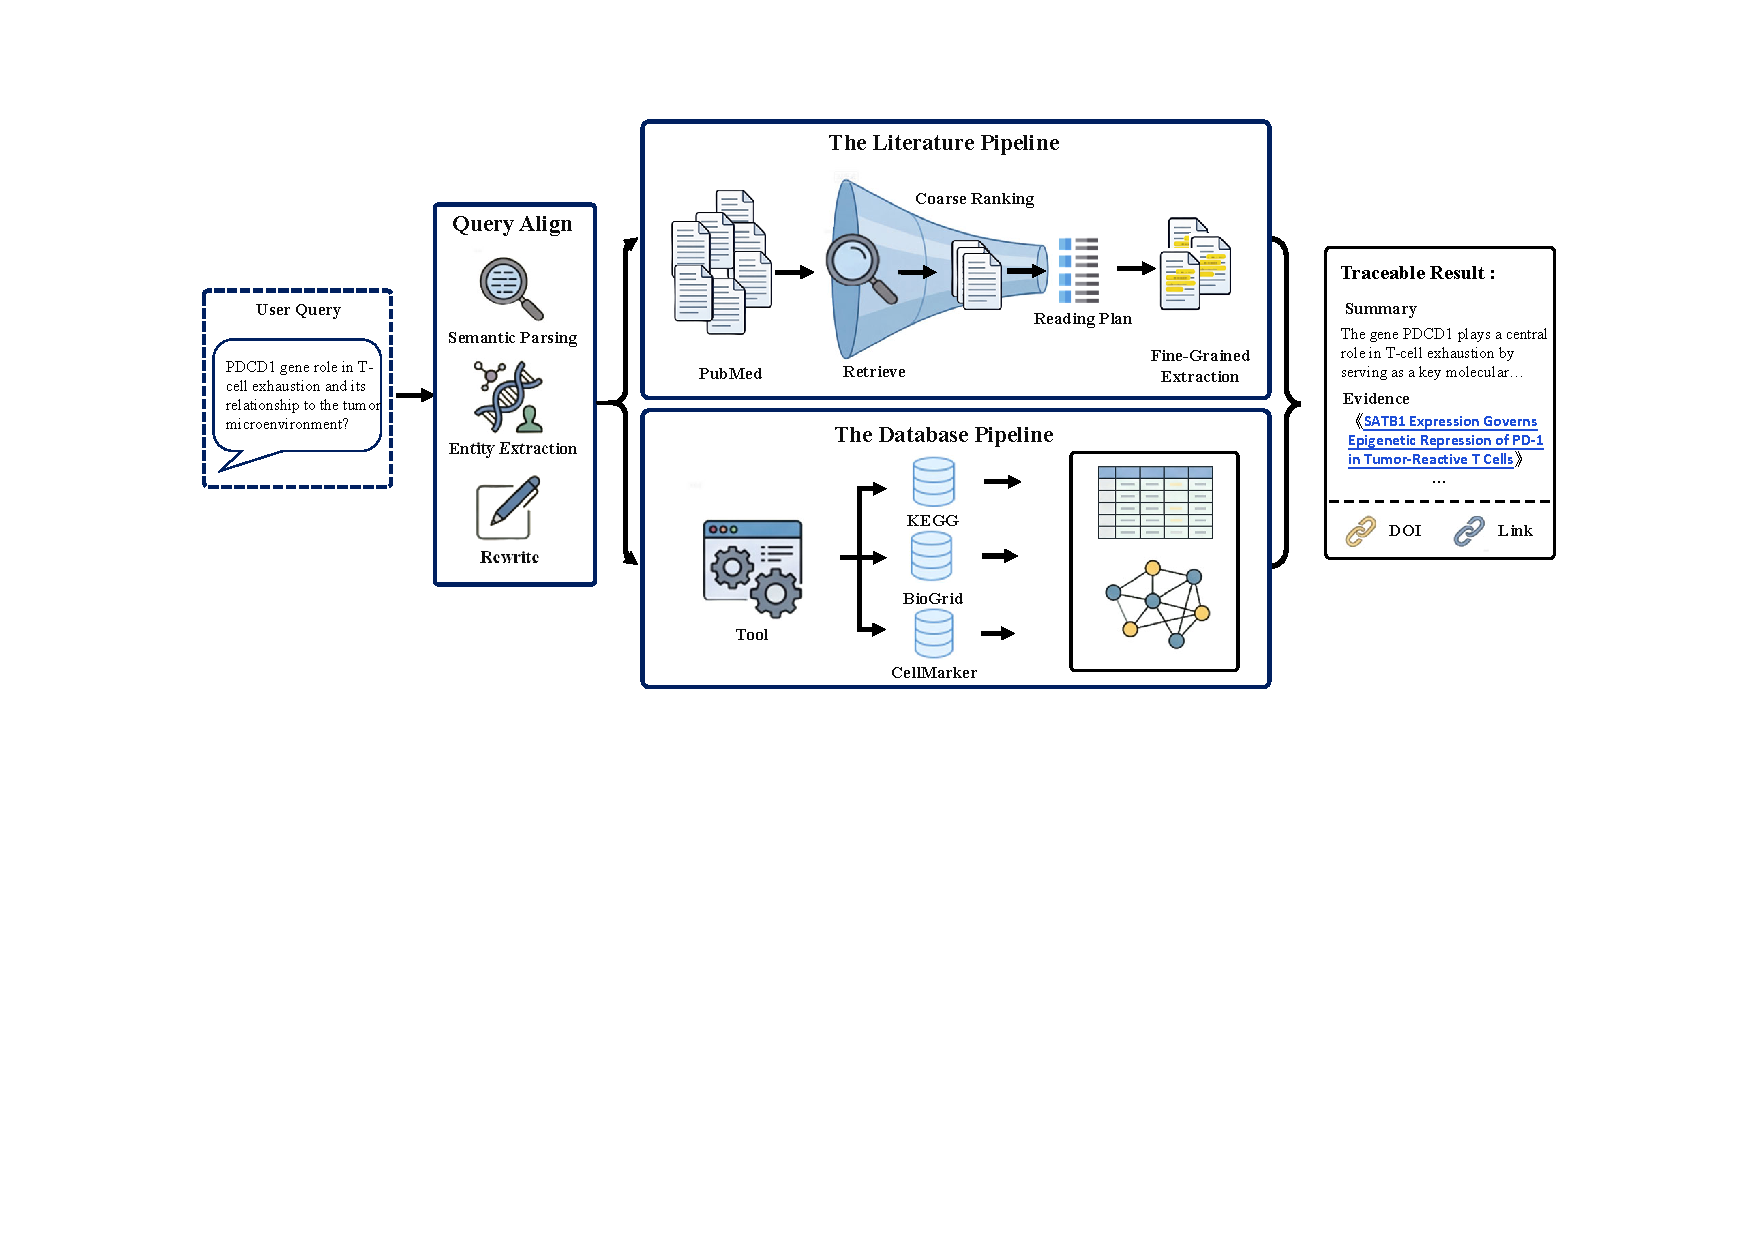
\includegraphics[width=1\linewidth]{Knowledge Integration Agent.pdf}
    \caption{The architecture of Knowledge Integration Agent. The workflow proceeds from left to right, starting with the Query Alignment which standardizes ambiguous user inputs. The process then bifurcates into two complementary pipelines: (Top) The Literature Pipeline employs a RAG-based funnel to process massive unstructured text, using coarse ranking and a targeted reading plan to distill the top 50 candidates down to highly relevant evidence; (Bottom) The Database Pipeline directly retrieves structured molecular facts via unified APIs. Finally, information from both sources is synthesized into Traceable Insights, grounded with explicit citations (DOIs, URLs) to support downstream verification and reasoning.}
    \label{fig:KIA}
\end{figure*}

\subsection{Data Interpretation Agent (DIA): Multi-Modal Understanding and Synthesis}

DIA is designed to interpret computational outputs during spatial transcriptomics analysis. As illustrated in \textbf{Figure \ref{fig:Data-Interpretation-Agent}}, the agent operates in two distinct modes to accommodate different analytical granularities: \textbf{(A) Single File Query} for specific data inspection, and \textbf{(B) File Tree Query} for complex, multi-file synthesis.

\textbf{Single File Query Mode:} As shown in \textbf{Figure \ref{fig:Data-Interpretation-Agent}(A)}, the agent possesses multi-modal capabilities to handle diverse file formats individually. It accepts user queries targeting specific outputs, such as identifying significant genes from CSV files, analyzing variable genes in AnnData objects (H5AD), or interpreting visualization plots (e.g., UMAP, spatial maps). By leveraging code generation tools and Multi-modal Large Language Models (MLLMs), the agent extracts statistical metrics and visual features to provide precise, isolated answers.

\textbf{File Tree Query Mode:} This mode is designed for comprehensive assessments that require synthesizing information across an entire execution record. Instead of indiscriminately reading all files, which risks context overflow, the agent employs a dynamic \textbf{Reorder Plan} to logically sequence data access based on the query's intent. As illustrated by the Quality Control (QC) validation example in \textbf{Figure \ref{fig:Data-Interpretation-Agent}(B)}, this plan prioritizes the workflow: first extracting core parameters, then validating numerical results, and finally seeking supporting evidence from plots (e.g., Violin plots). This structured approach enables the agent to aggregate fragmented evidences into a cohesive synthesis, ensuring that the final conclusion is both biologically interpretable and statistically robust.

% The agent's specific processing logic for different file types ensures accuracy across both modes:
% \begin{itemize}
%     \item \textbf{Text files (Reports)}: Targeted extraction of core conclusions and experimental design parameters, summarizing content to focus on key analysis indicators.
%     \item \textbf{Structured data files (e.g., CSV, AnnData):} Combined with file content previews, the agent automatically generates Python code to query structured data, converting complex numerical matrices into human-readable insights regarding gene expression and variability.
%     \item \textbf{Image files (Plots)}: Utilizing vision-language capabilities, the agent objectively interprets visual patterns (e.g., cluster separation in UMAP, distribution in QC plots). The reading plan aligns these visual interpretations with numerical data to perform cross-validation, strictly describing biological implications without hallucination.
% \end{itemize}

To ensure analytical accuracy across both modes, the agent applies tailored logic to seamlessly handle diverse file types. When processing text reports, it targets the extraction of core conclusions and experimental design parameters, condensing the content to focus strictly on key analytical indicators. For structured data, such as CSV or AnnData files, the agent couples file previews with automated Python code generation to query the data, effectively translating complex numerical matrices into human-readable insights on gene expression and variability. Furthermore, when analyzing image files like plots, it leverages advanced vision-language capabilities to objectively interpret visual patterns—such as UMAP cluster separation or distributions in QC plots. By aligning these visual interpretations with numerical data for rigorous cross-validation, the agent accurately delineates biological implications while strictly preventing hallucinations. Ultimately, this unified approach enables the agent to synthesize text, numerical matrices, and images, delivering a comprehensive analysis of heterogeneous data.

This design, centered on ordered reading plans, effectively enables multi-file joint analysis while maintaining system stability. It ensures that the agent’s contextual reasoning remains precise, reduces the cognitive burden on users, and delivers interpretable, high-quality results that directly support biological hypothesis generation and validation.


\subsection{Knowledge Integration Agent (KIA): Contextualization of Results with External Biological Knowledge}

KIA is designed to resolve a critical bottleneck in spatial transcriptomics analysis: the interpretation of computational results (e.g., region-specific gene expression patterns) is often constrained by a lack of external biological context. Unlike conventional tools limited to isolated analytical findings, KIA automates the retrieval, synthesis, and cross-validation of high-relevance external knowledge, thereby streamlining the validation of biological plausibility without requiring manual literature synthesis.

% 生物医学查询往往包含多实体（基因、通路、疾病等）、多约束（物种、实验条件、时间窗口等）与模糊语义，传统检索工具难以精准提取核心意图，易出现“漏检关键实体”或“误判约束条件”的问题，导致检索结果与研究需求偏差较大。
% 两类数据都有特点，数据库中（快速提供明确的分子互作结论）准确稳定，但是可能存在滞后，而文献数据（提供实验证据、语境约束与前沿进展）碎片化（查询可能得到大量语境相近但是与问题无关的文献）
Biological knowledge sources exhibit inherent heterogeneity and complementary utility. Structured biological databases (e.g., CellMarker, BioGrid, KEGG, NichNet) provide relatively precise and stable conclusions regarding molecular interactions, though they may occasionally suffer from curation lags. In contrast, academic literature offers timely experimental evidence, specific contextual constraints, and cutting-edge insights. However, the utility of literature is often challenged by its massive volume and unstructured nature. The vast quantity of textual data, combined with high information density, makes rapid information extraction and systematic reading computationally demanding for human researchers.


The workflow of KIA is driven by two parallel pipelines initiated by a query alignment module. Biomedical queries typically involve complex semantics with multiple entities (e.g., genes, pathways, diseases) and constraints (e.g., species, experimental conditions). To address this, KIA first performs query alignment to parse the semantic context, extracting core entities and constraints. The original query is then rewritten into a standardized format. This preprocessing ensures retrieval accuracy and mitigates deviations caused by ambiguous semantics.

% 对于文献数据，我们充分利用现有RAG进展，实现了检索改写，粗排，精排，读取过程。我们首先对于重写问题再次改写为pubmed的高级查询语句，检索到相关文献后，再使用reranker模型对于重写后的查询进行排序，粗排掉前50篇文献，之后再通过整体读取，生成读取计划（选择最关键的5篇），读取计划包括对于每一篇文献需要关注的关键内容，分别读取后，收集相关证据
The first pipeline targets unstructured literature data by leveraging advanced Retrieval-Augmented Generation (RAG) technology \cite{lewis2020retrieval}. The rewritten query is optimized into PubMed advanced search syntax to narrow the search scope within the massive literature pool. Following initial retrieval, a reranker model performs relevance sorting to filter noise, retaining the top 50 documents in a coarse-ranking stage. To efficiently tackle the challenge of reading unstructured text, KIA generates a targeted \textit{reading plan}. This plan selects the 5 most critical documents and defines specific extraction objectives (e.g., gene-pathway interaction evidence, experimental methods) for each. This strategy transforms the broad scanning of unstructured text into a focused extraction of high-value evidence, ensuring systematic cross-validation.
% 对于数据库数据，我们收集了来自于xxxxx的数据（可能可以列个表、cellmarker、biogrid、kegg、nichnet）等，并提供统一接口，由agent自用户改写数据中提取关键实体后进行调用查询
The second pipeline focuses on structured data, integrating multi-source biological databases. Upon extracting core entities from the standardized query, KIA autonomously invokes corresponding database interfaces to retrieve structured knowledge (e.g., gene regulatory networks from BioGrid, pathway annotations from KEGG). 

% 最后对于多源数据总结得到结果，
Finally, KIA synthesizes knowledge obtained from both pipelines to enhance interpretability. The retrieved information is organized logically: background context $\rightarrow$ supportive evidence (dual-source) $\rightarrow$ supplementary explanations. This structured synthesis explicitly links external knowledge to in-house experimental results, enabling users to rapidly discern connections between spatial transcriptomics findings and existing research, thereby facilitating hypothesis generation.
% 意义
A defining characteristic of KIA is the strict \textbf{traceability of biological evidence}. All integrated external knowledge is presented with granular source attribution, including manuscript titles, contextual excerpts, URLs, and Digital Object Identifiers (DOIs). This transparency serves a dual purpose. First, it facilitates human verification, allowing researchers to directly access original sources for rapid fact-checking and citation during manuscript preparation. Second, and crucially, it establishes a verifiable ground truth for inter-agent collaboration. Downstream agents, such as the Orchestrator Agent and Data Interpretation Agent, utilize this evidence as a reference framework to evaluate analytical outcomes—specifically, assessing the concordance between observed spatial expression patterns and reported mechanisms, or identifying potential discrepancies that may spark novel biological findings.

% 后续再添加关于前端页面的章节（感觉不用为其写results）


\section{Results}

We evaluated STAnalyzer on two representative spatial transcriptomics datasets spanning different platforms and resolutions to validate its end-to-end analytical capabilities, biological interpretability, and cross-platform scalability: (1) a spot-level 10x Visium human DLPFC dataset (3,673 spots, 33,538 genes) for assessing automated analysis and biological consistency with known cortical architecture, and (2) a subcellular-resolution 10x Xenium human lung cancer dataset (161,000 cells, 480 genes) for demonstrating scalability and the capacity for hypothesis-driven biological discovery.
% This section aims to verify the core capabilities of the STAnalyzer framework: converting users' advanced natural language queries into executable atomic analysis services, and accurately parsing the unstructured computational results produced by these services at the semantic level, thereby structuring the computational outputs into inferable biological information.

% \textbf{Service Planner Agent Bridging Natural Language Queries to Atomic Bioinformatic Functions:}
% The traditional ST analysis process requires users to have the ability to convert high-level research intentions into specific API calls at the lower level, which often leads to workflow fragmentation and technical barriers. The SPA aims to solve this problem by implementing intelligent scheduling for atomic analysis services. The core of SPA is context-awareness, which can automatically infer and configure the optimal parameters required for the service to run based on the current data state and user requirements.

% We verified the scheduling accuracy and parameter decision-making capability of SPA through a typical function enrichment analysis task.
% \begin{quote}
% \emph{User Query : ``Perform functional enrichment analysis on the DEG list of cluster to identify highly relevant signaling pathways, prioritizing human databases."}

% \emph{Context Files : ``spatial\_cluster\_data.h5ad"}
% \end{quote}
% \textbf{1. Service Selection and Matching}

%  SPA autonomously analyzes the user request and selects the optimal service from its repository:
% \begin{quote}
% \emph{Service Planner Agent: ``The user query requests a functional enrichment analysis on the DEG list of clusters to identify relevant signaling pathways, with a focus on human databases. The `gene-enrichment-analysis' service is specifically designed for cluster-based gene enrichment analysis using clustered spatial transcriptomics data in AnnData format, which matches the provided context file. The input file (spatial\_cluster\_data.h5ad) contains cluster labels and gene expression data required by this service. No prior execution history exists, so this step has not been attempted. This service is the most appropriate to fulfill the user's request directly."}
% \end{quote}
% \textbf{2. Intelligent Parameter Configuration}

% After service selection,  SPA translates the nuanced semantic constraints into precise parameter settings.
% \begin{quote}
% \emph{Service Planner Agent: ``The user requested functional enrichment analysis on the DEG list of clusters with a focus on signaling pathways and prioritization of human databases. To best meet this goal, `gene\_selection\_method' was set to `marker\_genes' (instead of the default `top\_expressed') to specifically capture differentially expressed genes (DEGs) that define each cluster, which is more appropriate for DEG-based enrichment. The `library' was changed to 'KEGG\_2021\_Human' to prioritize signaling pathways (KEGG is pathway-centric) and use the most recent human-specific database. `organism' remains 'Human' as required. The `engine' is kept as \gx{`enrichr' [enricher?]} since it supports KEGG\_2021\_Human via Enrichr's library access. `top\_n\_genes' is omitted as it is only relevant when using `top\_expressed'. This configuration avoids defaults where better choices exist per the task and ensures human-focused, pathway-relevant results."}
% \end{quote}

% % 感觉可以写的再简单一些
% In summary, the SPA's parameter decision-making process is as follows:

% \begin{itemize}
%     \item \textbf{Pathway and Organism Focus:} The request for ``signaling pathways" and ``human databases" leads to the precise configuration of the `library' as $\text{`KEGG\_2021\_Human'}$ and the `organism' as $\text{`Human'}$.
%     \item \textbf{DEG List Interpretation:} The request to analyze the ``DEG list of cluster" is accurately interpreted as a need to analyze genes defining specific cell states. This prompts the SPA to set the `gene\_selection\_method' to $\text{`marker\_genes'}$, overriding a potential default of top-expressed genes, which is less biologically appropriate for cluster-specific functional analysis.
%     \item \textbf{Redundant Parameter Exclusion:} The `top\_n\_genes' parameter is correctly omitted as it is only relevant for the alternative $\text{`top\_expressed'}$ method.
% \end{itemize}
% This comparison validates the SPA's capability to precisely convert the user's semantic constraints into the exact parameter values, demonstrating its ability to achieve high-precision service scheduling under complex constraints, thereby significantly eliminating the need for researchers to manually select tools and configure intricate parameters.

% \textbf{Data Interpretation Agent: Semantic Structuring and Quality Assessment of Heterogeneous Outputs:}
% Following the successful service by SPA, DIA executes the next critical step: semantic-level interpretation and quality assessment of the service outputs. The DIA's role is not to  merely display the raw results but to integrate information from heterogeneous files (raw statistical tables, log files, and visualizations) and transform them into actionable biological insights, while also evaluating the quality of the analytical step itself.

% We demonstrate the DIA's robust interpretation capability on the output of the functional enrichment service (Case Study I). The analysis yielded 938 enriched terms across six clusters, generating multi-modal outputs including a CSV table, a summary text file, bar plots (\text{`enrichment\_bar.png'}), and volcano plots (\text{`enrichment\_volcano.png'}).

% \textbf{1. Structural Interpretation and Statistical Contextualization:}
% The DIA successfully read and structured the statistical data, revealing a scarcity of significant findings: only $2$ terms ($0.21\%$) achieved statistical significance ($\text{adjusted } P < 0.05$) across all clusters. The overall distribution of adjusted P-values ($\text{mean}=0.8501$, $\text{median}=0.8827$) corroborated a minimal level of significance across the dataset. Crucially, DIA identified a severe limitation in the underlying biological signal: the mean gene overlap per enriched pathway was only $1.73$ ($\text{median}=1.00$), suggesting limited confidence in pathway-level interpretations due to shallow input depth.

% \textbf{2. Multi-Modal Semantic Integration for Interpretation:}
% The DIA integrated insights across statistical reports and visual representations. It identified that only \textbf{Cluster 4} contained statistically significant results, pinpointing \textbf{``Ether lipid metabolism"} and \textbf{``PI3K-Akt signaling pathway"} ($\text{adjusted } P=0.0217$). This finding was validated by cross-referencing three independent outputs:
% \begin{itemize}
%     \item The \textbf{CSV/Summary} data reported the minimum adjusted P-value and the two significant terms in Cluster 4.
%     \item The {\textbf{Volcano Plots} where only the plot corresponding to Cluster 4 showed data points above the significance threshold.}
%     \item The \textbf{Spatial Coherence Assessment} linked the statistical finding back to the underlying data quality, noting that Cluster 4 exhibited notably lower spatial variance \gx{($\text{X variance} \approx 1.09 \times 10^6$) [$10^{-6}$?]}, suggesting it is a spatially cohesive and biologically distinct region, thereby lending credibility to its unique enrichment signal.
% \end{itemize}
% The integration confirmed that the biological signal was strongly localized to a single, spatially coherent domain (Cluster 4).

% \textbf{3. Result Quality Assessment and Feedback Loop:}
% Beyond interpretation, the DIA performed an essential quality check, evaluating the analytical step based on the outcome sparsity. The finding of only two significant terms prompted DIA to generate a feedback summary (Execution Quality Summary), suggesting that the low yield might be due to ``overly stringent corrections" or ``suboptimal marker gene selection". This mechanism represents the first component (\textbf{self-correction closed-loop}) of STAnalyzer, demonstrating the system's ability to assess execution quality and potentially trigger re-planning or parameter adjustment for subsequent steps.

% Collectively, DIA demonstrates a robust capacity to transform heterogeneous computational outputs into structured, validated, and context-rich biological conclusions, a prerequisite for advanced knowledge integration and automated hypothesis generation.

% STAnalyzer执行读取文献分析
% \subsection{STAnalyzer Achieving Deep Contextualization via Robust Integration of Literature Knowledge}
% This section aims to verify the capability of STAnalyzer to integrate information from external knowledge bases, enabling \textbf{literature-supported deep contextualization} of biological explanations for analytical results. This integration thereby enhances the scientific value and readability of analysis reports.

% We demonstrate the capability of KIA by tasking it to address a high-level biological question centered on \textit{PDCD1}—a key gene identified in the ST data.

% \textbf{1. Targeted Query Execution and Intelligent Rewriting:} 

% The Knowledge Integration Agent (KIA) initiates its workflow by receiving a high-level, targeted functional query. This query can be directly initiated by a researcher or automatically triggered by an upstream analytical agent (e.g., following the identification of $\textit{PDCD1}$ as a significant differentially expressed gene in the ST analysis).

% \begin{quote}
% \emph{User Query: "What is the role of the gene PDCD1 in T-cell exhaustion and how is it related to the tumor microenvironment?"}
% \end{quote}

% To optimize retrieval from external knowledge bases, KIA first performs an intelligent query rewriting step, converting the natural language question into a concise, keyword-rich format that maximizes search engine relevance.

% \begin{quote}
% \emph{Rewrite Query: "PDCD1 gene role in T-cell exhaustion and its relationship to the tumor microenvironment?"}
% \end{quote}

% \textbf{2. Knowledge Retrieval, Ranking, and Filtering}

% KIA executes the rewritten query against external knowledge bases. To ensure high contextual relevance, it employs a multi-step filtering process:

% \begin{itemize}
%     \item \textbf{Initial Retrieval:} KIA retrieves an initial set of documents (e.g., 50 documents) from the knowledge base using the rewritten query.
%     \item \textbf{Relevance Ranking and Filtering: } These 50 documents are passed through a context-aware reranker model. This model scores each document based on its deep semantic relationship to the user's specific query. Based on these scores, KIA selects only the top-ranked, most relevant subset of literature (e.g., the top 20 documents) for subsequent, detailed analysis, effectively reducing noise.
% \end{itemize}

% \textbf{3. Dynamic Reading Plan and Focused Extraction}

% KIA develops a dynamic ``reading plan" for the filtered literature, ensuring that the extraction process is goal-oriented, targeting the specific mechanistic details required to answer the user's query comprehensively. For each of the top-ranked documents, KIA formulates a specific reading objective. For example, for the document relevant to T-cell exhaustion signatures, we only present the key segments here:

% \begin{quote}
% \emph{Title: T-cell exhaustion interrelates with immune cytolytic activity to shape the inflamed tumor microenvironment.}

% \emph{Reading Objective: Extract information about the role of PDCD1 in defining the transcriptional signature of T-cell exhaustion, its correlation with immune cytolytic activity (CYT), and how this shapes the inflamed tumor microenvironment. Also, identify how PDCD1 expression relates to response to immune checkpoint inhibitors.}

% \end{quote}
% KIA executes this plan by extracting key snippets, such as the finding that a 78-gene signature for exhausted $\text{CD8}^+ \text{T}$ cells (GET) was defined using $\text{PD-1-high}$ vs. $\text{PD-1-negative}$ cells, and that this GET signature (with $\textit{PDCD1}$ as a marker) correlates with intratumoral CYT \cite{cai2020t}.

% \textbf{4. Synthesis and Comprehensive Biological Narrative}

% By executing these focused reading plans across the top literature, KIA synthesizes the extracted information into a coherent, comprehensive answer. This structured output directly addresses the multifaceted nature of the original query, transforming raw data context into a rich biological narrative.

% \begin{quote}
% \emph{\textbf{Final Answer:} ``The gene $\textit{PDCD1}$ plays a central role in T-cell exhaustion and significantly influences the tumor microenvironment (TME) across multiple cancer types. $\textit{PDCD1}$ encodes the programmed cell death protein 1 (PD-1), a key immune checkpoint receptor expressed on activated T cells, whose interaction with PD-L1 on tumor cells within the TME drives T-cell exhaustion, leading to impaired proliferative capacity, reduced cytotoxic function, and diminished cytokine secretion. This process is a hallmark of dysfunctional anti-tumor immunity, as detailed in literature such as 'Reversing T Cell Exhaustion by Converting Membrane PD-1 to Its Soluble form in Jurkat Cells...'"}
% \end{quote}
% This comprehensive approach validates  KIA's ability to automate the translation of a high-level biological question into a precise, multi-faceted, cited, and mechanistically rich answer, significantly enhancing the scientific rigor of ST data interpretation.




\subsection{STAnalyzer enables rapid, biologically interpretable automated analysis of spatial transcriptomics}


%% spot/单细胞和亚细胞精度【人类脑切片/head and neck cancer data】, 小规模/大规模   (两个case强调不同平台，不同规模，都能够进行分析)

% 为了展示STAnalyzer在ST数据上完整的对话式自动分析能力及其实用价值，我们将其应用在10x Genomics Visium human DLPFC dataset【1】。该数据集包含3,673 spots 和 33,538 gene，我们首先输入“Please perform data preprocessing on this slice and briefly describe the quality of the processed data” 展开数据的预处理分析。STAnalyzer会自动进行初步的数据统计分析（Figure.5a），并采用合适的方式执行预处理操作得到质控后的数据。结果显示处理后的数据保留了3234 spots 和 19877 gene (Figure .5a)，执行的策略选择与参数设置均显示地展示在对话框，并且从Robust filtering，Biologically plausible QC profiles，Consistent multi-format validation和Analysis-ready output四个层面给出总结报告评估此次预处理的质量，供用户决策。进一步地，我们输入“Please identify the spatial domain of this data and briefly assess the rationality of the resulting spatial domain division”，STAnalyzer将数据划分为了8个空间域，呈现出清晰的层次结构 (Figure.5b)。更重要的是，STAnalyzer会对划分结果给出评估与反馈，比如在结果统计上提到“Domain counts (n = 8) and size distribution (195–665 spots) reflect biologically interpretable granularity—not overly fragmented nor excessively coarse”，在视觉层面提到“domain_umap.png confirms transcriptional separability in low-dimensional embedding, with high intra-domain compactness and only minor, localized inter-domain overlap”。如果评估结果出现负面意见，用户可以根据反馈重新执行该步骤，得到更有意义的生物结果。

% 接着，我们执行了一个综合分析，提问道：“Based on the obtained 8 spatial domain division results, execute the relevant services to analyze the functional characteristics of each domain. Finally, please provide a table summarizing what each domain is and its corresponding functional characteristics”。STAnalyzer自动规划步骤，执行了四个层面的分析来完成这一过程。首先，对每个域进行了Spatial TF Activity Scoring与spatial metabolic pathway activity 服务，鉴别了每个域得分最高的top基因以及 top代谢通路，图5c,d展示的是活性得分较高的基因和通路，主要集中在EGR1, NFIC, ATFF6, RORA, SP1, TAL1几个人脑组织特异性相关基因，以及与能量供给，突触传递，多巴胺相关的代谢通路，这与已知的关于人 DLPFC 的正常生理代谢的相关研究保持一致【3，4，5】。此外，细胞类型注释与GO富集分析的结果也表现出生物合理性，比如细胞类型主要集中在神经细胞和少突胶质细胞【6】。最后，基于得到的多维度证据，STAnalyzer执行自动的证据交叉验证 (Figure. 5g)，通过内部一致性检验以及多证据的定位，确定每个空间域的功能特征，其中四个域很好的匹配上已知的生物学标注 (Figure. 5h)。比如域0与xxx相关【7，8，9，10】。值得注意的是，即使是在这种用户0先验提供的情况下（系统预先不知道输入的是什么组织的数据，也不知道应该划分为几个空间域），STAnalyzer通过多智能体协作能够完美匹配上人类脑切片数据的空间结构与功能特征，展现其实际应用价值。此外，这种多维度验证分析只需要在几分钟内就可全部完成，并提供详细可追溯的证据支撑，大大加速了科研分析进程。

% 除此之外，用户也可以一步到位直接输入“Please analyze what functional characteristics this data possesses”进行全自动分析，STAnalyzer也会将任务拆解为一整套透明可执行的流程（比如数据预处理，空间域识别等等），然后逐步执行分析，最后给出分析报告与证据支撑。不过这种方式相比半自动方式，缺少了更直观的中间过程的智能体反馈与用户逐步干预，人机交互弱一些，优点是更便捷。



To demonstrate the comprehensive conversational automated analysis capabilities and practical utility of STAnalyzer for spatial transcriptomics data, we applied the framework to the 10x Genomics Visium human dorsolateral prefrontal cortex (DLPFC) dataset \cite{maynard2021transcriptome}. Comprising 3,673 spots and 33,538 genes, the analysis commenced with the prompt: ``Please perform data preprocessing on this slice and briefly describe the quality of the processed data." STAnalyzer automatically executed preliminary statistical profiling (Fig. \ref{case1}a) and selected optimal preprocessing strategies to generate quality-controlled data. The processed dataset retained 3,234 spots and 19,877 genes (Fig. \ref{case1}a). Crucially, the chosen strategies and parameter settings were explicitly displayed in the dialogue interface. The system provided a summary report evaluating preprocessing quality across four dimensions—Robust filtering, Biologically plausible QC profiles, Consistent multi-format validation, and Analysis-ready output, thereby facilitating informed user decision-making. Subsequently, upon receiving the instruction ``Please identify the spatial domain of this data and briefly assess the rationality of the resulting spatial domain division" STAnalyzer segmented the tissue into eight spatial domains, revealing a distinct hierarchical architecture (Fig. \ref{case1}b). Notably, the system provided autonomous evaluation and feedback on the segmentation results. Statistically, it noted that ``Domain counts ($n$=8) and size distribution (195–665 spots) reflect biologically interpretable granularity—not overly fragmented nor excessively coarse." Visually, it confirmed that the ``domain\_umap.png confirms transcriptional separability in low-dimensional embedding, with high intra-domain compactness and only minor, localized inter-domain overlap." Should the evaluation yield negative feedback, users can iteratively refine and re-execute this step based on the system's suggestions to ensure biologically meaningful outcomes.

We then proceeded to a comprehensive functional characterization by prompting: ``Based on the obtained 8 spatial domain division results, execute the relevant services to analyze the functional characteristics of each domain. Finally, please provide a table summarizing what each domain is and its corresponding functional characteristics". STAnalyzer autonomously orchestrated {a comprehensive multi-dimensional analysis pipeline}. First, it performed Spatial TF Activity Scoring and spatial metabolic pathway activity analysis for each domain. Fig. \ref{case1}c,d illustrate the top-ranked genes and pathways, highlighting the robust activity of brain-enriched transcription factors (e.g., EGR1, NFIC, ATF6, RORA, SP1, and TAL1) and the significant enrichment of pathways associated with energy metabolism, synaptic transmission, and dopaminergic signaling. These findings closely align with the established physiological and metabolic profiles of the human DLPFC. For instance, EGR1 and RORA are well-documented to be pivotal for synaptic plasticity and neuronal survival in the prefrontal cortex \cite{duclot2017role,sarachana2013genome}. Similarly, the prominent activity in energy supply and dopamine metabolism pathways is a hallmark of the DLPFC, underpinning its complex executive functions and working memory capabilities \cite{magistretti2015cellular,cools2011inverted}. Furthermore, cell type annotation and Gene Ontology (GO) enrichment analyses demonstrated biological plausibility, with cell types predominantly identified as neurons and oligodendrocytes \cite{maynard2021transcriptome}. Leveraging this multi-dimensional evidence, STAnalyzer executed an automated evidence cross-validation process (Fig. \ref{case1}g). Through internal consistency checks and multi-evidence triangulation, it defined the functional identity of each spatial domain. Four domains exhibited precise alignment with known biological annotations of the human prefrontal cortex (Fig. \ref{case1}h). For instance, Domain 0 was defined as the myelinated white matter core, driven by oligodendrocyte-specific myelination and oxidative phosphorylation \cite{stadelmann2019myelin}. Cortical neuronal niches were captured by Domain 1 and Domain 4, which highlighted dopaminergic synaptic transmission \cite{seamans2004principal} and neurotrophin-guided synaptic plasticity \cite{zeng2012large} in superficial layers, respectively. Moreover, the identification of a vascular-associated smooth muscle niche (Domain 3) accurately reflected the cerebrovascular architecture essential for cortical homeostasis \cite{iadecola2017neurovascular}. Notably, even without any prior tissue-type annotation or predefined domain count—where the system received no task-specific configuration regarding the input data, the multi-agent collaboration within STAnalyzer accurately reconstructed the spatial architecture and functional characteristics of the human brain slice. Moreover, this comprehensive multi-dimensional validation was completed within minutes, providing detailed, traceable evidentiary support that significantly accelerates the research workflow.

Alternatively, users can opt for a fully automated workflow by inputting a high-level directive such as ``Please analyze what functional characteristics this data possesses." In this mode, STAnalyzer decomposes the request into a transparent, executable sequence of tasks (e.g., data preprocessing, spatial domain identification), executes them sequentially, and generates a final report supported by evidence. While this approach offers greater convenience, it involves less human-in-the-loop interaction compared to the semi-automated mode, offering fewer opportunities for intuitive intermediate feedback and iterative user intervention.


%% spot精度，spot少，基因多
\begin{figure*}
    \centering
    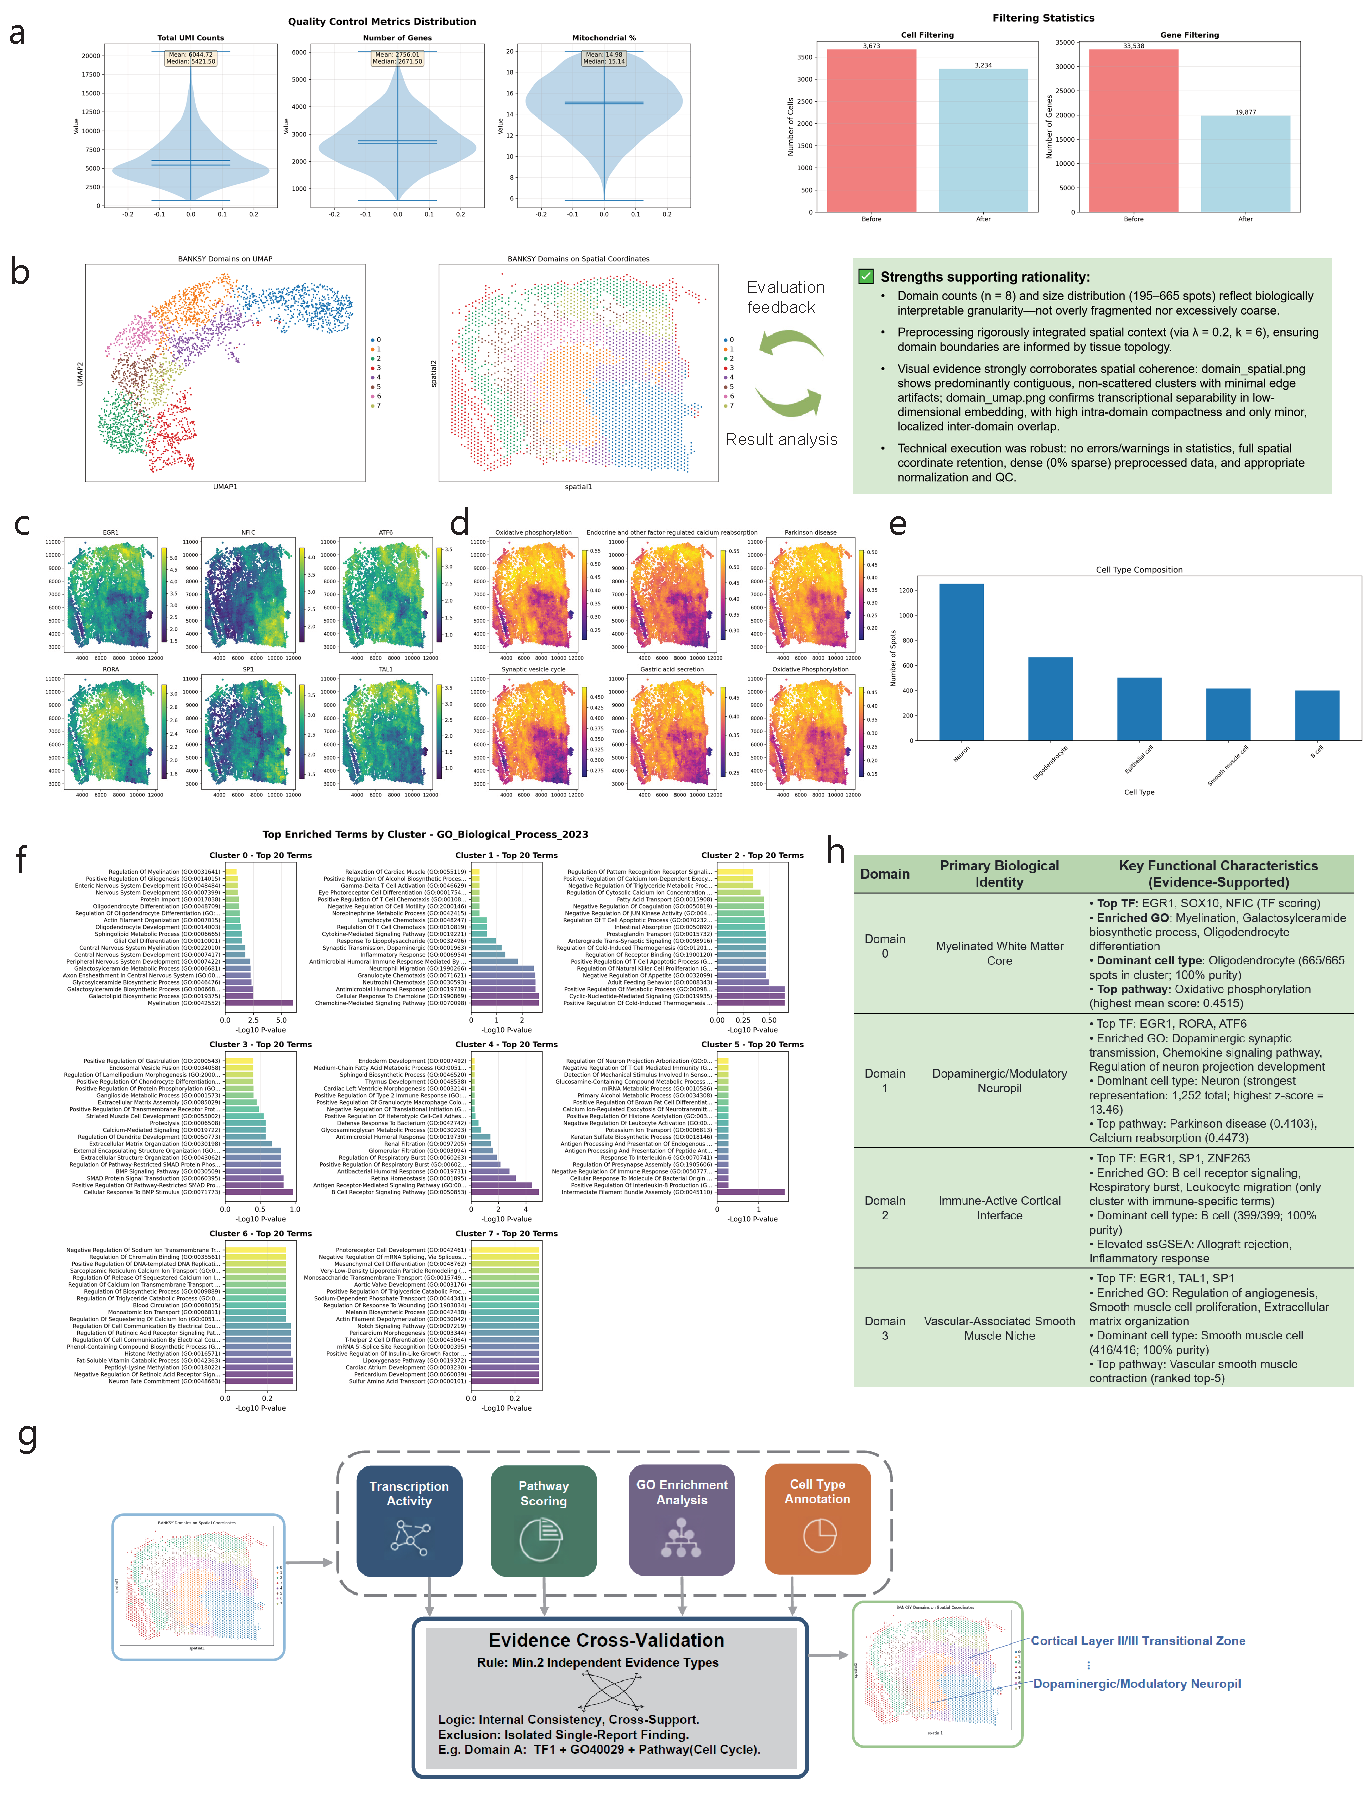
\includegraphics[width=0.95\linewidth]{./figure/case1.pdf}
    \caption{\textbf{Automated analysis on the human DLPFC dataset.} \textbf{a} (Left) Statistical analysis of various metrics of the original ST data. (Right) Bar chart of the number of cells and genes before and after quality control. \textbf{b} Spatial domain identification results and the automatic assessment feedback provided by STAnalyzer. \textbf{c} Heatmap of the top-6 TFs with high spatial TF activity scores. \textbf{d} Heatmap visualizing the spatial distribution of major enriched metabolic pathway activities across the ST data. \textbf{e} Bar plot of cell type composition. The chart displays the number of spatial spots assigned to each identified major cell type across the tissue section. \textbf{f} Top 20 enriched GO terms for each of the eight spatial domains. \textbf{g} STAnalyzer conducts evidence cross-validation at four levels to automatically analyze the functional characteristics of each spatial domain. \textbf{h} Traceable and interpretable functional characterization of four spatial domains, highly consistent with established biological knowledge.}
    \label{case1}
\end{figure*}


\subsection{STAnalyzer facilitates biological discovery via cross-platform automated analysis at subcellular resolution}

% 为了进一步展现STAnalyzer跨平台应用的可扩展性以及更高阶的科研探索能力，我们将其应用到一个亚细胞精度测序的10x Xenium 人类肺癌空转数据【1】。该数据集包含161000个亚细胞和480个基因，细胞数量规模是脑切片spot规模的近50倍，经过初步的预处理之后（Figure xx），执行自动化的空间域识别，得到包含9个空间域的极其致密、结构饱满的病理组织（Figure xx）。随后，我们输入自然语言“Please analyze the main cell type composition of each of the 9 spatial domains one by one（Each spatial domain contains more than one type of cell, and it is composed of multiple cell types）, and perform gene enrichment analysis for each domain. Finally, summarize the analysis results for each spatial domain in tabular form.” STAnalyzer自动执行分析并绘图获得了每个空间域的主要细胞类型组成（Figure xx）与主要富集terms （Figure xx）。基于此，我们通过提示词“Based on the cell type annotations and gene enrichment analysis results of these 9 spatial domains that have been completed, please further analyze and infer the functional domains that each spatial domain may belong to (provide explainable evidence). Finally, form a summary table to clearly display the characteristics of each spatial domain.”让其自动整合实验结果进行细粒度的功能划分，其中有两个值得关注的现象，第一，STAnalyzer刻画了 Domain 3 这一呈现连续带状的空间域，空间图谱与功能分析（显著富集 regulation of T cell activation 和 T cell tolerance induction，且高表达 FOXP3, TGFB1）显示 （Figure xx），Domain 3 是一个由 Treg 细胞主导的免疫抑制物理界面（Immunosuppressive interface）。这直观地揭示了肿瘤是如何在空间上构建物理屏障，将具有杀伤力的 T 细胞阻挡在核心区之外的【2】。第二，STAnalyzer将复杂的免疫浸润区解构为两个功能迥异但空间相邻的微环境：Domain 0 和 Domain 1 (Figure xx and xx)。功能分析显示，Domain 0 富集了 T 细胞激活通路（CD3D/E, IL2RA），代表抗原经历过的 T 细胞微环境；而 Domain 1 则高度富集 B 细胞激活与体液免疫通路（CD19, MS4A1）。这种细胞毒性免疫与体液免疫在物理空间上的相邻与分区（Zonation），高度提示了类似三级淋巴结构（TLS）或异位淋巴滤泡的形成【3】。这证明STAnalyzer不仅能识别细胞类型，更能自动化地解析复杂的高级免疫空间拓扑结构。

% 为了展现STAnalyzer在亚细胞精度下通过多智能体协作加速新的可解释的生物学发现的潜力，我们注入提示：“The current dataset possesses a truly accurate resolution of subcellular physical coordinates. Our previous analysis has successfully identified a crucial physical communication boundary: Domain 0 (the core of adaptive immunity dominated by T cells) and Domain 3 (the immunosuppressive barrier dominated by Tregs). Please focus on the interface where physical contact occurs between Domain 0 and Domain 3 (the boundary). From the perspective of subcellular analysis, deduce and extract potential new biological discoveries. Please conduct a deep analysis using an explainable thought chain (Chain of Thought).”。STAnalyzer自动写代码，并且综合文件元数据、决策历史以及成功建立的知识基础中所获取的所有可用证据，自动提出深度的、基于机制的推理结果，并且都有可追溯的思维链与结果文件 （Figure xx），而不是虚无的捏造，大大减少了大模型幻觉的产生【6】。STAnalyzer的综合分析结果指出：“The Domain 0/Domain 3 interface is not a passive diffusion barrier, but an active, organelle-engineered decision hub, where: (i)Physical contact triggers asymmetric mitochondrial trafficking to enforce metabolic compartmentalization; (ii)CTLA4, LAG3, and TIGIT operate not as isolated receptors, but as nanoscale organizers of endocytic, actin, and lysosomal machinery; (iii)Tunneling nanotubes mediate directional, suppressive mitochondrial transfer, converting T cells into transiently anergic effectors via cGAS–STING — a boundary-specific, non-apoptotic immune silencing mechanism. This reframes the immunosuppressive barrier not as static cellular segregation, but as a dynamic, subcellularly orchestrated interface — offering new targets for precision immunomodulation (e.g., inhibiting TNT formation in autoimmunity, or enhancing mitochondrial transfer in cancer immunotherapy).”。基于上述的亚细胞空间分析，重新定义了域0/3之间的 immunosuppressive barrier not as static cellular segregation, but as a dynamic, subcellularly orchestrated interface — offering new targets for precision immunomodulation (e.g., inhibiting TNT formation in autoimmunity, or enhancing mitochondrial transfer in cancer immunotherapy)，这在之前的研究中存在部分侧面互补的报道xxx【7,8】，进一步说明了STAnalyzer在加速新的生物学发现方面的潜力。总的来说，我们也许不能完全把STAnalyzer当作一种科研发现的金标准，但是它通过多智能体协作可以在数十分钟之类完成超过10万细胞数量的亚细胞层面的空转分析，并且提供基于证据的，可解释的生物学发现，这对降低科研门槛，提高生物发现的信心、以及寻找新的科学问题具有重大意义。


To further demonstrate the cross-platform scalability and advanced exploratory capabilities of STAnalyzer, we applied it to a subcellular-resolution 10x Xenium spatial transcriptomics dataset of human lung cancer \cite{janesick2023high,blampey2025novae}. Comprising over 161,000 cells and 480 genes, this dataset represents a cellular scale nearly 50-fold larger than that of brain slice spots. Following initial preprocessing (Fig. \ref{case2}a), automated spatial domain identification was executed, yielding a highly dense and structurally intact pathological tissue representation comprising nine distinct spatial domains (Fig. \ref{case2}b). Subsequently, we inputted the natural language query: ``Please analyze the main cell type composition of each of the 9 spatial domains one by one (Each spatial domain contains more than one type of cell, and it is composed of multiple cell types), and perform gene enrichment analysis for each domain. Finally, summarize the analysis results for each spatial domain in tabular form." STAnalyzer automatically executed the analysis and generated plots, detailing significantly enriched terms (Fig. \ref{case2}c) and the primary cell type composition (Fig. \ref{case2}d) and for each spatial domain.

Building upon this, we prompted the system to automatically integrate the experimental results for fine-grained functional compartmentalization: ``Based on the cell type annotations and gene enrichment analysis results of these 9 spatial domains that have been completed, please further analyze and infer the functional domains that each spatial domain may belong to (provide explainable evidence). Finally, form a summary table to clearly display the characteristics of each spatial domain". Notably, two compelling phenomena emerged from this analysis. First, STAnalyzer delineated Domain 3 as a continuous, band-like spatial region. Spatial mapping and functional analysis (which showed significant enrichment for the regulation of T cell activation and T cell tolerance induction, alongside high expression of FOXP3 and TGFB1) revealed that Domain 3 constitutes an immunosuppressive physical interface dominated by regulatory T (Treg) cells (Fig. \ref{case2}e). This intuitively illustrates how tumors spatially construct physical barriers to exclude cytotoxic T cells from the core region \cite{joyce2015t,schurch2020coordinated}. Second, STAnalyzer deconstructed the complex immune infiltration region into two functionally distinct yet spatially adjacent microenvironments: Domain 0 and Domain 1 (Fig. \ref{case2}b, e). Functional analysis indicated that Domain 0 is enriched for T cell activation pathways (CD3D/E, IL2RA), representing an antigen-experienced T cell microenvironment. Conversely, Domain 1 is highly enriched for B cell activation and humoral immune pathways (CD19, MS4A1). This spatial adjacency and zonation of cytotoxic and humoral immunity strongly suggests the formation of tertiary lymphoid structures (TLS) or ectopic lymphoid follicles \cite{sautes2019tertiary}. Collectively, these findings demonstrate that STAnalyzer can not only identify cell types but also autonomously decipher complex, higher-order topological structures within the immune spatial microenvironment.


To demonstrate the potential of STAnalyzer in accelerating new, interpretable biological discoveries at the subcellular level through multi-agent collaboration, we provided the following prompt: ``The current dataset possesses a truly accurate resolution of subcellular physical coordinates. Our previous analysis has successfully identified a crucial physical communication boundary: Domain 0 (the core of adaptive immunity dominated by T cells) and Domain 3 (the immunosuppressive barrier dominated by Tregs). Please focus on the interface where physical contact occurs between Domain 0 and Domain 3 (the boundary). From the perspective of subcellular analysis, deduce and extract potential new biological discoveries. Please conduct a deep analysis using an explainable thought chain (Chain of Thought)." STAnalyzer autonomously generated code and synthesized all available evidence extracted from file metadata, decision history, and the established knowledge base to propose in-depth, mechanism-based inferences. Crucially, these insights are supported by traceable chains of thought and output files (Fig. \ref{case2}f), ensuring they are firmly grounded in data rather than being baseless fabrications, thereby significantly mitigating the occurrence of large language model hallucinations \cite{yao2022react}. The comprehensive analysis by STAnalyzer concluded: ``The Domain 0/Domain 3 interface is not a passive diffusion barrier, but an active, organelle-engineered decision hub, where: (i) Physical contact triggers asymmetric mitochondrial trafficking to enforce metabolic compartmentalization; (ii) CTLA4, LAG3, and TIGIT operate not as isolated receptors, but as nanoscale organizers of endocytic, actin, and lysosomal machinery; (iii) Tunneling nanotubes mediate directional, suppressive mitochondrial transfer, converting T cells into transiently anergic effectors via cGAS–STING — a boundary-specific, non-apoptotic immune silencing mechanism. This reframes the immunosuppressive barrier not as static cellular segregation, but as a dynamic, subcellularly orchestrated interface — offering new targets for precision immunomodulation (e.g., inhibiting TNT formation in autoimmunity, or enhancing mitochondrial transfer in cancer immunotherapy)." Based on the aforementioned subcellular spatial analysis, the immunosuppressive barrier between Domain 0 and Domain 3 is characterized not as static cellular segregation, but as a dynamic, subcellularly orchestrated interface (Fig. \ref{case2}g). This perspective offers novel targets for precision immunomodulation (e.g., inhibiting TNT formation in autoimmunity, or enhancing mitochondrial transfer in cancer immunotherapy). Notably, these computationally derived hypotheses share complementary parallels with recent experimental evidence \cite{baldwin2024intercellular,kwon2020cytosolic}, further illustrating the capacity of STAnalyzer for cross-platform automated analysis and accelerated biological discovery.

In conclusion, while computational predictions made by STAnalyzer cannot replace rigorous experimental validation as the gold standard for biological discovery, it serves as a valuable tool for generating high-confidence hypotheses. By autonomously executing subcellular spatial transcriptomic analysis of over 100,000 cells within tens of minutes, it transforms massive datasets into evidence-based, interpretable insights. This framework lowers the technical barrier to complex computational research, provides reliable starting points for experimental design, and offers a practical engine for cross-platform automated analysis and accelerated biological discovery.


\begin{figure*}
    \centering
    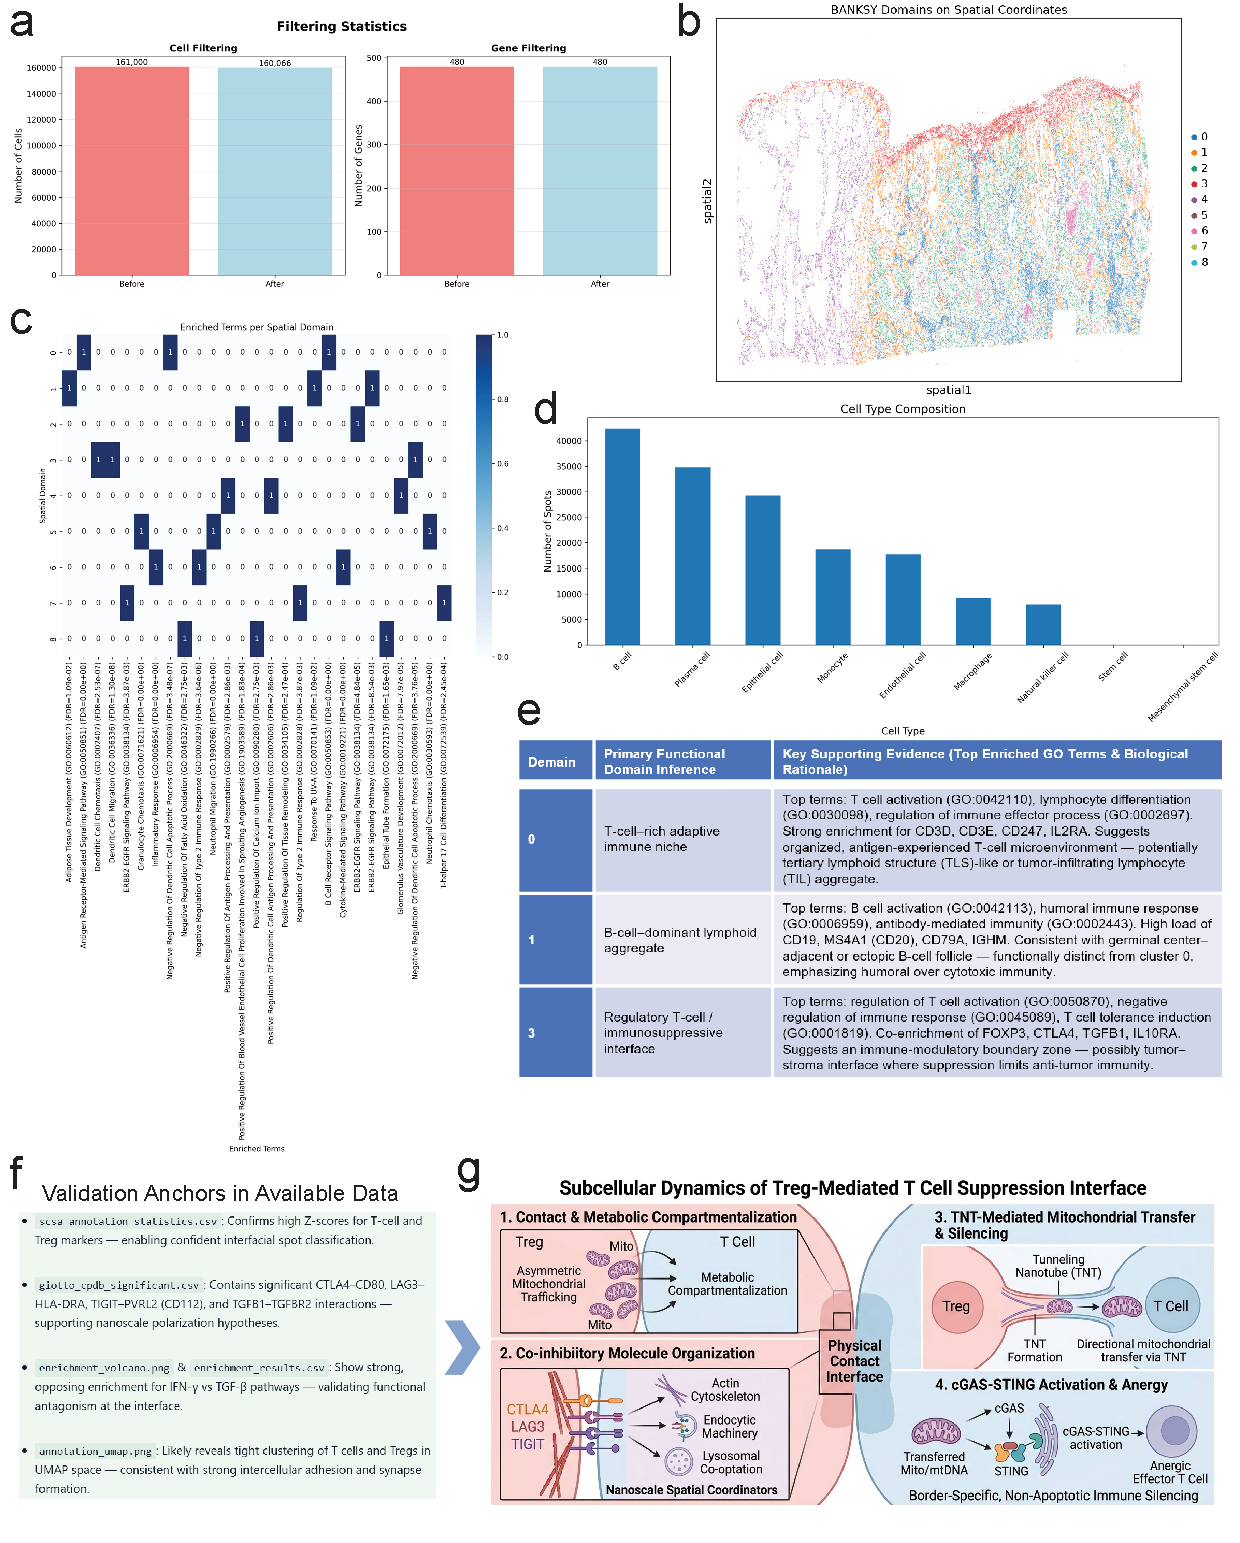
\includegraphics[width=0.95\linewidth]{./figure/case2.pdf}
    \caption{\textbf{Extended experiments on the 10x Xenium human lung cancer dataset.} \textbf{a} Bar chart of the number of cells and genes before and after quality control. \textbf{b} Spatial domain identification results by STAnalyzer. \textbf{c} Heatmap of the top 3 GO terms enriched in each spatial domain. \textbf{d} Bar plot of cell type composition. The chart displays the number of spatial spots assigned. \textbf{e} The inferred functional results of the main spatial domain and the explainable supporting evidence. \textbf{f} STAnalyzer automatically formulates new biological hypotheses based on the available direct evidence. \textbf{g} Subcellular dynamics of the Treg-mediated immunosuppressive interface. The physical boundary between Tregs and T cells acts as an active signaling hub. Contact-driven spatial reorganization of co-inhibitory molecules and TNT-mediated mitochondrial transfer synergistically activate the cGAS-STING pathway in T cells. This triggers non-apoptotic immune silencing (anergy), redefining the static barrier as a dynamic target for precision immunomodulation.}
    \label{case2}
\end{figure*}


\section{Discussion}
Spatial transcriptomics has revolutionized our understanding of tissue biology by linking gene expression to spatial context, yet the translation of high-dimensional ST data into actionable biological insights remains hindered by fragmented toolchains, steep technical barriers, and the disconnect between computational results and biological knowledge. In this study, we present STAnalyzer, an intelligent multi-agent framework that addresses these critical gaps through a Human-in-the-Loop (HITL) collaborative architecture, integrating intent-driven orchestration, multi-modal self-refinement, and evidence-based cross-validation. Here, we discuss the core contributions, comparative advantages, limitations, and future directions of STAnalyzer, as well as its broader implications for the field of spatial omics analysis.

Unlike ``black-box" pipelines or isolated agents, STAnalyzer’s four specialized agents collaborate to automate end-to-end analysis while retaining human oversight. Key innovations include robust execution via constraint-based tool matching and containerization, semantic integration of multimodal outputs, and dual-pipeline (literature/database) knowledge integration—resolving fragility, multimodal blindness, and epistemic isolation in existing tools. The HITL paradigm balances automation with human intuition, empowering non-computational researchers to leverage ST analysis without sacrificing control or transparency. Practically, STAnalyzer democratizes access to spatial transcriptomics by substantially lowering computational barriers and ensuring reproducibility through traceable, evidence-based reporting. Crucially, the framework exhibits exceptional cross-platform scalability, seamlessly adapting from macroscopic tissue profiling (e.g., analyzing thousands of spots via 10x Visium) to the subcellular-resolution mapping of massive cellular cohorts (e.g., over 100,000 cells via 10x Xenium). By successfully navigating diverse and complex biological contexts—ranging from neuroarchitecture to precision oncology—STAnalyzer drastically reduces manual analytical workloads. Ultimately, it serves as a robust engine for cross-platform automated analysis and accelerated biological discovery, streamlining rapid hypothesis generation and evidence synthesis.

Limitations include a current focus on standard 2D transcriptomic tasks, with future work needed to expand coverage to spatial multi-omics and 3D modalities; reliance on static knowledge sources, which will require real-time synchronization mechanisms; and potential usability gaps for novice users. Future directions involve expanding the tool library, integrating real-time knowledge updates, simplifying user interactions, optimizing distributed computing for ultra-large datasets, and enhancing robustness to noisy data. Ultimately, STAnalyzer represents a paradigm shift toward collaborative intelligence in spatial omics, bridging computational efficiency with biological relevance to drive cross-platform automated analysis and accelerated biological discovery.

As ST technologies continue to evolve, intelligent analytical frameworks will play an increasingly important role in translating spatial data into biological discoveries \cite{williams2022introduction}. STAnalyzer provides a robust, user-friendly solution for end-to-end ST analysis, and ongoing refinements will strengthen its utility as a versatile tool in spatial omics research.

\section{Webserver Implementation}
STAnalyzer is built as a high-performance, scalable web service, designed specifically to support complex multi‑agent collaborative workflows and the processing of large-scale ST data. The backend adopts a microservices architecture, containerized with Docker for isolation and scalability, and uses FastAPI on Uvicorn for high‑concurrency, low‑latency APIs. MongoDB handles structured logs and metadata, while network file systems manage large raw and intermediate data. Intelligent orchestration is powered by LangChain and LangGraph, with Qwen integration for natural language understanding and dynamic decision-making. Tasks are executed asynchronously—each receives a unique Execution ID, and real‑time progress is streamed to the frontend via Server‑Sent Events. The frontend is a Vue 3‑based single‑page application using TypeScript and Vite, with Element Plus for UI consistency and Pinia for state management. Interactive workflow visualizations are rendered with AntV G6, and analytical charts are generated using Apache ECharts. Token-based authentication ensures security without requiring manual password entry., and the platform is fully compatible with modern browsers (Chrome, Firefox, Edge, Safari), providing researchers with an interactive interface for data exploration, real‑time visualization, and result download.

\section{Data availability}
The STAnalyzer platform is publicly accessible at \href{https://www.sdu-idea.cn/STAnalyzer}{https://www.sdu-idea.cn/STAnalyzer}, with no registration or access restrictions for academic and non-commercial use.
% {ProteoWeb is publicly available at \href{https://www.sdu-idea.cn/ProteoWeb}{https://www.sdu-idea.cn/ProteoWeb}, without the need of registration or login.} 



\section{Acknowledgement}
%This work is supported by National Key Research and Development Program (No. 2023YFF0725500 and 2024YFF1206604) and National Natural Science Foundation of China (No. 62531013, 62432006 and 62272276),  Natural Science Foundation of Shandong Province (ZR2024JQ001 and ZR2025LZH004) and Taishan Scholars Program (tsqn202408317).

\section{Funding}
This work is supported by National Key Research and Development Program (No. 2023YFF0725500 and 2024YFF1206604) and National Natural Science Foundation of China (No. 62531013, 62432006 and 62272276),  Natural Science Foundation of Shandong Province (ZR2024JQ001 and ZR2025LZH004) and Taishan Scholars Program (tsqn202408317).

\subsubsection{Conflict of interest statement.} 
None declared.
% \newpage


% \bibliographystyle{natbib}
\bibliographystyle{unsrt}
\bibliography{NAR-bib}



% \begin{thebibliography}{4}

% % Format for article
% % \bibitem{1}
% % Author,A.B. and Author,C. (1992)
% % Article title.
% % \textit{Abbreviated Journal Name}, \textbf{5}, 300--330.
% % 
% % Format for book
% % \bibitem{2}
% % Author,D., Author,E.F. and Author,G. (1995)
% % \textit{Book Title}.
% % Publisher Name, Publisher Address.
% % 
% % Format for chapter in book
% % \bibitem{3}
% % Author,H. and Author,I. (2005)
% % Chapter title.
% % In
% % Editor,A. and Editor,B. (eds),
% % \textit{Book Title},
% % Publisher Name, Publisher Address,
% % pp.\ 60--80.
% % Format for chapter in book
% % 
% % Another article
% % \bibitem{4}
% % Author,Y. and Author,Z. (2002)
% % Article title.
% % \textit{Abbreviated Journal Name}, \textbf{53}, 500--520.

% \end{thebibliography}

\end{document}
